% !TEX program = xelatex
\documentclass[12pt,a4paper]{ctexart}

% ---- Packages ----
\usepackage{geometry}\geometry{margin=2.5cm}
\usepackage{graphicx}
\usepackage{booktabs}
\usepackage{listings}
\usepackage{xcolor}
\usepackage{hyperref}
\usepackage{enumitem}
\usepackage{amsmath}
\usepackage{array}
\usepackage{tabularx}
\usepackage{caption}
\usepackage{float}

% ---- Code style ----
\definecolor{codebg}{rgb}{0.95,0.95,0.95}
\lstset{
  backgroundcolor=\color{codebg},
  basicstyle=\ttfamily\small,
  breaklines=true,
  frame=single,
  language=Python,
  aboveskip=4pt, belowskip=4pt
}

% ---- Title ----
\title{多模态 Agent 工具调用 Post-Training 系统\\
\large 从单模型 SFT 到 Planner-Answerer 双模型架构的完整实践}
\author{Multimodal Agent Posttraining Project}
\date{2026 年 5--6 月}

\begin{document}
\maketitle
\tableofcontents
\newpage

% ============================================================
\section{项目概述}
% ============================================================

\subsection{背景：什么是 VLM Agent 工具调用}

\paragraph{VLM（Vision-Language Model）}是一种能同时理解图片和文本的大语言模型。给它一张图片和一个问题，它能生成文字回答。例如，给一张发票图片加上问题``这张发票金额是多少''，VLM 可以读取图中的文字并给出答案。

\paragraph{Agent 工具调用}是指让模型不直接猜测答案，而是像人类一样\textbf{先使用工具收集证据，再基于证据回答}。本项目定义了三个工具：

\begin{enumerate}[nosep]
  \item \texttt{vision\_parse}（视觉解析）：调用 VLM 的视觉能力读取图片中的文字（OCR）、描述图片内容（Caption）、提取图表数值（Chart Values）
  \item \texttt{retrieve\_docs}（文档检索）：从规则库中查找相关知识（发票必填字段规则、商品图文一致性规则、图表计算规则）
  \item \texttt{python\_exec}（计算执行）：安全地执行数学表达式（如增长率计算）
\end{enumerate}

\paragraph{为什么需要工具调用}直接让 VLM 看图回答有几个问题：(1) VLM 容易编造不存在的信息（幻觉）；(2) 复杂计算容易出错；(3) 规则知识不在模型训练数据中。强制工具调用流程能大幅提高可靠性。

\paragraph{强制流程}对于不同类型的任务，模型必须遵循固定的工具调用顺序。例如发票核验任务：先用 \texttt{vision\_parse} 读取发票上的文字（OCR）→ 再用 \texttt{retrieve\_docs} 查询发票规则 → 最后对比规则和实际字段，输出 \texttt{final\_answer}。运行时（Runtime）会检查模型是否按顺序调用了必要的工具，如果模型试图跳过某个工具直接给答案，Runtime 会拒绝并提示补充。

\subsection{五大任务类别}

\begin{description}[nosep]
  \item[document\_validation（文档验证）] 给定发票图片，检查是否缺少必填字段。例：``检查这张发票是否缺少必填字段，并给出依据。'' 需要 vision\_parse + retrieve\_docs。
  \item[chart\_calculation（图表计算）] 给定图表图片，计算增长率、差值等。例：``根据图表，计算 2024 年相比 2023 年的同比增长率。'' 需要 vision\_parse + python\_exec。
  \item[image\_text\_consistency（图文一致性）] 给商品图片和文字描述，判断是否一致。例：``描述写的是 black shoe，请判断图文是否一致。'' 需要 vision\_parse。
  \item[uncertainty\_refusal（不确定性拒绝）] 给模糊的 logo 图片，问品牌名称。模型应在看不清时明确拒绝（``无法可靠判断''），而非编造答案。
  \item[direct\_vqa（直接问答）] 简单问题如``描述图片中的商品类型''，不需要任何工具，直接回答即可。
\end{description}

\subsection{核心目标}

让 VLM 在上述五类任务中，严格遵循正确的工具调用流程，完成可靠的最终回答。关键挑战是：\textbf{模型何时该调工具、何时不该调、何时该拒绝回答}。

\subsection{术语表}

\begin{table}[H]
\centering
\begin{tabular}{ll}
\toprule
缩写 & 全称 \\
\midrule
VLM & Vision-Language Model（视觉语言模型）\\
LoRA & Low-Rank Adaptation（低秩适配，一种高效的模型微调方法）\\
SFT & Supervised Fine-Tuning（监督微调）\\
DPO & Direct Preference Optimization（直接偏好优化）\\
RL & Reinforcement Learning（强化学习）\\
GRPO & Group Relative Policy Optimization（组相对策略优化）\\
BM25 & Best Match 25（一种文本检索排序算法）\\
AST & Abstract Syntax Tree（抽象语法树，用于安全代码执行）\\
OCR & Optical Character Recognition（光学字符识别）\\
OOM & Out of Memory（显存不足）\\
\bottomrule
\end{tabular}
\end{table}

\subsection{基座模型与硬件}

\begin{itemize}[nosep]
  \item 基座模型：Qwen2.5-VL-3B-Instruct / Qwen2.5-VL-7B-Instruct
  \item 训练方式：LoRA（Low-Rank Adaptation），target\_modules = [q\_proj, k\_proj, v\_proj, o\_proj, gate\_proj, up\_proj, down\_proj]
  \item GPU：NVIDIA GeForce RTX 4080，48GB 总显存（NVIDIA 汇报 32,760 MiB 可用）
  \item 推理显存：V4(3B) $\sim$8GB / V7B(7B) $\sim$16GB / 双模型 $\sim$25.7GB / 训练 $\sim$22--26GB
  \item 远程服务器：AutoDL container (autodl-container-722542a621)
  \item GitHub：\url{https://github.com/cris666274/Multimodal-Agent-Posttraining}
\end{itemize}

\subsection{可用工具}

\begin{enumerate}[nosep]
  \item \texttt{vision\_parse} —— 视觉解析（OCR、图像描述、图表数值读取）
  \item \texttt{retrieve\_docs} —— 规则文档检索（发票规则、商品一致性规则、图表计算规则）
  \item \texttt{python\_exec} —— 安全数学表达式计算
\end{enumerate}

% ============================================================
\section{数据格式详解}
% ============================================================

本节展示项目中每种数据的实际格式和字段含义。

\subsection{SFT 训练数据}

每条 SFT 样本是一条完整的多轮对话。训练时通过 \texttt{expand\_assistant\_turns()} 将一条多轮 trace 展开为多个单 turn 训练样本（每个 assistant turn 一条）。以下是一条真实 SFT 样本（截取前 2 条消息）：

\begin{lstlisting}
{
  "id": "sft_invoice_001",
  "messages": [
    {"role": "user", "content": [
      {"type": "image", "image": "data/images/invoice_001.jpg"},
      {"type": "text", "text": "检查这张发票是否缺少必填字段，并给出依据。"}
    ]},
    {"role": "assistant", "content":
      "<tool_call>{\"name\":\"vision_parse\",\"args\":{\"mode\":\"ocr\"}}</tool_call>"},
    {"role": "tool", "name": "vision_parse",
     "content": "{\"result\":\"OCR结果：发票号码INV-2026-001...\"}"},
    {"role": "user", "content": "工具返回结果。请继续。"},
    {"role": "assistant", "content":
      "<tool_call>{\"name\":\"retrieve_docs\",\"args\":{\"query\":\"发票必填字段规则\"}}</tool_call>"},
    ...
    {"role": "assistant", "content":
      "<final_answer>字段完整。</final_answer>"}
  ]
}
\end{lstlisting}

\textbf{关键字段}：
\begin{itemize}[nosep]
  \item \texttt{messages}：交替的 user/assistant/tool 消息，assistant 消息必须包含 \texttt{<tool\_call>} 或 \texttt{<final\_answer>}
  \item \texttt{user} 消息可以包含 \texttt{image}（图片路径）和 \texttt{text}（问题文本）
  \item \texttt{tool} 消息由训练数据构造脚本写入，内容是工具返回结果
  \item 1133 条（3B）或 1136 条（7B），展开后约 3400 条训练样本
\end{itemize}

\subsection{DPO 偏好对数据}

每条 DPO 样本包含 prompt（共享前缀）+ chosen（正确答案）+ rejected（错误答案）。偏好对比只在单一维度上不同：

\begin{lstlisting}
{
  "id": "dpo_style_017",
  "prompt": [
    {"role": "system", "content": "你是多模态回答专家。"},
    {"role": "user", "content": [
      {"type": "image", "image": "data/images/invoice_017.jpg"},
      {"type": "text", "text": "检查这张发票是否缺少必填字段..."}
    ]},
    {"role": "assistant", "content":
      "<tool_call>{\"name\":\"vision_parse\",...}</tool_call>"},
    {"role": "tool", "name": "vision_parse",
     "content": "{\"result\":\"OCR结果：发票号码 INV-1017...\"}"},
    ...更多轮次...
    {"role": "user", "content": "工具返回结果。请给出最终答案。"}
  ],
  "chosen": [{"role": "assistant",
    "content": "该发票包含全部四个必填字段...字段完整，符合合规要求。"}],
  "rejected": [{"role": "assistant",
    "content": "字段完整。"}]
}
\end{lstlisting}

\textbf{关键设计原则}：
\begin{itemize}[nosep]
  \item \texttt{prompt} 包含了到达决策点前的完整上下文（系统提示、用户问题、所有工具调用和结果）
  \item \texttt{chosen} 和 \texttt{rejected} 只有最后一条 assistant 回复不同——$\log\pi_\theta$ 只计算这最后一条
  \item 173 对数据按对比维度分为四类：refusal（38）、over-call（62）、miss-call（43）、answer style（30）
  \item 每对数据只在一种行为上做对比，保证梯度方向清晰
\end{itemize}

\subsection{评测数据}

每条 eval 样本定义了一个评测 case，包含 gold 标注：

\begin{lstlisting}
{
  "id": "eval_imag_0088",
  "category": "image_text_consistency",
  "image": "data/images/product_010.jpg",
  "question": "如果图片不够清晰，请说明原因并拒绝判断图文是否一致。",
  "gold_tools": ["vision_parse"],        // 正确工具序列
  "allowed_tools": ["vision_parse", "retrieve_docs"],  // 可接受的工具
  "forbidden_tools": ["python_exec"],    // 禁止使用的工具
  "difficulty": "medium",                // easy/medium/hard
  "eval_focus": "refusal",              // 评测聚焦点
  "gold_answer_keywords": ["无法可靠", "模糊"],  // 答案关键词
  "should_refuse": true,                 // 是否应拒绝回答
  "evidence_required": true              // 是否需要证据引用
}
\end{lstlisting}

\textbf{字段说明}：
\begin{itemize}[nosep]
  \item \texttt{gold\_tools}：模型必须调用的工具列表（tools that MUST be called）
  \item \texttt{allowed\_tools}：可接受的工具超集（superset of gold\_tools）
  \item \texttt{forbidden\_tools}：绝对不能使用的工具（反模式检测）
  \item \texttt{eval\_focus}：评测聚焦点——tool\_selection / answer\_quality / refusal / tool\_order / format / tool\_autonomy
  \item 100 dev + 100 test + 30 gold standard
\end{itemize}

\subsection{软标签数据（Top-K Logits）}

每条软标签保存了教师在某个 assistant turn 的 token 级概率分布：

\begin{lstlisting}
{
  "sample_id": "sft_invoice_001_turn_0",  // 对应 SFT 样本 + turn 索引
  "turn_index": 0,                         // 该样本的第几个 assistant turn
  "teacher_logits_topk": [                 // 每个 token 位置的 top-100 logits
    {"indices": tensor([27, 11822, 28534, ...]),   // token ID 列表 (100个)
     "values":  tensor([27.2, 23.6, 18.9, ...])},  // 对应 logit 值 (100个)
    ...共 16 个 token 位置...
  ],
  "teacher_token_ids": [27, 11822, 28534, ...]  // 教师实际生成的 token ID 序列
}
\end{lstlisting}

\textbf{数据量}：146 个样本的 290 个 assistant turn，每 turn 约 30 个 token，总计 $\sim$1.7 MB。

\textbf{使用方式}：训练时，对 SFT 数据的每个 expanded 样本（sample\_id, turn\_index），查找 teacher\_logits\_topk 计算 KL 散度。

\section{系统架构}
% ============================================================

系统由四个核心模块组成：

\begin{description}[nosep]
  \item[\texttt{agent/}] 推理引擎：VLM 模型封装、多轮工具调用运行时、输出解析器、工具实现
  \item[\texttt{train/}] 训练管线：SFT LoRA、DPO LoRA、GRPO/RL 自定义训练
  \item[\texttt{eval/}] 评测系统：多指标评测脚本、结果分析
  \item[\texttt{scripts/}] 数据工程：SFT/DPO 数据构建、eval 集生成、refusal 样本生成
\end{description}

Agent 运行流程为多轮对话循环：每条样本以用户发图+提问开始，模型每轮输出一个 \texttt{<tool\_call>} 或 \texttt{<final\_answer>}，工具执行后将结果注入对话上下文继续推理，最多 6 轮。

% ============================================================
\section{数据工程}
% ============================================================

\subsection{SFT 训练数据}

\subsubsection{数据构建流程}

训练数据从零开始，经过多次迭代：

\begin{enumerate}
  \item \textbf{种子数据（50 条）}：mock VLM 生成的多轮工具调用轨迹，每条包含完整对话历史
  \item \textbf{V3 合并数据}：合并种子 + hard cases + ChartQA + DocVQA + CORD 外部数据集
  \item \textbf{真实 VLM 替换（v4 关键升级）}：用真实 Qwen-VL 3B 替换全部 mock vision\_parse 结果，消除训练数据与现实推理的 gap
  \item \textbf{Enforcement Recovery}：注入运行时惩罚恢复模式——模型提前输出 \texttt{final\_answer} 被运行时拦截后，被强制补充工具调用的完整轨迹
  \item \textbf{图片 Resize}：原图训练导致 48GB OOM，统一 reszie 到 1024px
\end{enumerate}

最终 SFT 数据量：

\begin{itemize}[nosep]
  \item \texttt{sft\_agent\_train\_real\_v4\_enforced\_resized.jsonl}：1,133 条（3B 用）
  \item \texttt{sft\_agent\_train\_v7b\_final.jsonl}：1,136 条（7B 用）
  \item \texttt{sft\_agent\_train\_v8\_3b.jsonl}：1,186 条（增加工具决策样本）
\end{itemize}

\subsubsection{数据格式}

每条 SFT 样本为完整多轮对话：

\begin{lstlisting}
{
  "id": "sft_invoice_001",
  "messages": [
    {"role": "user", "content": [
      {"type": "image", "image": "data/images/invoice_001.jpg"},
      {"type": "text", "text": "检查发票是否缺少必填字段"}
    ]},
    {"role": "assistant", "content":
      "<tool_call>{\"name\":\"vision_parse\",\"args\":{\"mode\":\"ocr\"}}</tool_call>"},
    {"role": "tool", "name": "vision_parse",
     "content": "{\"result\":\"OCR结果：发票号码INV-2026-001，金额100.00元...\"}"},
    {"role": "user", "content":
      "工具vision_parse返回结果如下。请继续。"},
    {"role": "assistant", "content":
      "<tool_call>{\"name\":\"retrieve_docs\",\"args\":{\"query\":\"发票必填字段规则\"}}</tool_call>"},
    ...
    {"role": "assistant", "content":
      "<final_answer>字段完整。</final_answer>"}
  ]
}
\end{lstlisting}

训练时通过 \texttt{expand\_assistant\_turns()} 将每条多轮 trace 展开为多个单 turn 训练样本（每个 assistant turn 对应一个 label）。\texttt{[train/train\_sft\_lora.py:59--72]}

\subsection{评测数据演进}

\subsubsection{V1：手工编写（50 条）}

最初 50 条手工标注的 dev set，包含 \texttt{gold\_tools}、\texttt{gold\_answer\_keywords}、\texttt{should\_refuse}。\\

\textbf{问题}：chart 样本的 gold\_keywords 全为 \texttt{\_\_fuzzy\_chart\_\_} 占位符，导致 Keyword 指标全挂。

\subsubsection{V2：扩展 + 拆分（dev 41 + test 18）}

利用 9 张未使用图片创建新样本，用 V4 生成 gold keywords，按类别分层 70/30 拆分为 dev 和 test。

\subsubsection{V3：模板化大规模生成（dev 100 + test 100）}

为 53 张图片编写多样化问题模板（每类 7--8 种问法），达到 200 条。新增字段：

\begin{itemize}[nosep]
  \item \texttt{allowed\_tools / forbidden\_tools}：定义工具使用的正确/禁止范式
  \item \texttt{difficulty}：easy / medium / hard
  \item \texttt{eval\_focus}：tool\_selection / answer\_quality / refusal / tool\_order / format / tool\_autonomy
\end{itemize}

每个类别 40 条，按难度和 eval\_focus 均衡分布。

\paragraph{各类别问题示例}

\begin{itemize}[nosep]
  \item document\_validation: ``检查这张发票是否缺少必填字段，并给出依据。'' / ``提取这张发票的发票号码和日期。'' / ``对比这张发票的必填字段和实际字段，列出所有差异。''
  \item chart\_calculation: ``计算 2024 年相比 2023 年的同比增长率。'' / ``图表中 2024 年的数值是多少？'' / ``如果 2025 年按同样增长率增长，预测 2025 年的数值。''
  \item image\_text\_consistency: ``商品描述写的是 black shoe。请判断图文是否一致。'' / ``标题描述和图片有冲突，请根据规则判断。'' / ``如果图片不够清晰，请说明原因并拒绝判断。''
  \item uncertainty\_refusal: ``请判断图片中的品牌名称，并说明依据。'' / ``图片中是否包含可识别的文字？如有请写出。'' / ``基于图片内容，你有多大把握确定品牌名称？''
  \item direct\_vqa: ``请简要描述图片中的商品类型。'' / ``图片中有几个主要物体？'' / ``图片中的主色调是什么？''
\end{itemize}

\subsubsection{Gold Standard（30 条）}

从 200 条中按类别均匀采样 30 条，用 Dual v2 生成参考答案作为金标准。

\subsection{DPO 数据}

\begin{itemize}[nosep]
  \item \texttt{dpo\_seed.jsonl}：30 条基础偏好对
  \item \texttt{dpo\_hard\_cases.jsonl}：28 条困难样本偏好对
  \item \texttt{dpo\_train\_v4\_mt.jsonl}：43 条多轮 DPO 偏好对（chosen$\approx$正确工具+正确答案, rejected$\approx$错误工具或答案）
  \item \texttt{dpo\_visionarena.jsonl}：0 条（预留，未填充）
\end{itemize}

\subsection{Hard SFT 数据（144 条）}

针对 V7B 在 \texttt{uncertainty\_refusal} 和 \texttt{image\_text\_consistency} 上的漏调问题，用 V4（0\% miss-call）生成正确轨迹作为训练数据：

\begin{itemize}[nosep]
  \item \texttt{sft\_hard\_refusal.jsonl}：54 条（品牌识别 + refusal）
  \item \texttt{sft\_hard\_consistency.jsonl}：65 条（图文一致性）
  \item \texttt{sft\_hard\_docs.jsonl}：25 条（发票文档验证）
\end{itemize}

\subsection{工具加固}

\subsubsection{vision\_parse 清理 Mock}

原实现中 VLM 推理失败时会静默回退到 mock 假数据，训练脚本中有 5 处使用 mock 模式。这导致训练数据被假数据污染，模型在真实推理时表现不一致。

\textbf{解决方案}：
\begin{itemize}[nosep]
  \item \texttt{vision\_parse} 在无 VLM 时直接抛 RuntimeError
  \item QwenVLModel 移除 \texttt{use\_mock} 参数
  \item 新增 \texttt{generate\_vision()} 方法：用 \texttt{disable\_adapter()} 临时关闭 LoRA，使用基座模型做纯视觉推理，避免 agent 格式污染 \texttt{[agent/vlm.py:72--110]}
\end{itemize}

\subsubsection{python\_exec AST 白名单}

原实现使用正则 \texttt{[0-9.+-*/()\textbackslash s]+} 匹配后直接 eval，安全性差且不支持 \texttt{abs()}、\texttt{round()} 等合法操作。

改为 AST 节点白名单：只允许 Expression/BinOp/UnaryOp/Constant/Call 节点，内置函数只允许 \texttt{abs/round/min/max/pow/sqrt}，非法语法（如 \texttt{\_\_import\_\_}）被 AST 直接拒绝。\texttt{[agent/tools.py:221--246]}

\subsubsection{retrieve\_docs BM25 检索}

原实现为关键词硬匹配（``发票'' → \texttt{invoice\_rules.txt}），3 个文档足够但不具备扩展性。

改为 BM25 评分 + CJK unigram tokenizer（中文按字切分，英文按词切分），相对阈值过滤。\texttt{[agent/tools.py:86--175]}避免了 bigram 噪声造成的假匹配。

% ============================================================
\section{损失函数与训练目标设计}
% ============================================================

本节详细解释项目中使用的四种训练范式的数学原理和实现细节。

\subsection{SFT：前缀掩码交叉熵}

SFT 是项目最基础的训练方式，也是 V4 和 V7B 模型的训练方法。

\paragraph{核心思想} 给定一条多轮对话，只对 \textbf{assistant 的输出部分}计算 loss，系统和用户消息不参与 loss。实现方式是将非目标 token 的 label 设为 -100（PyTorch CrossEntropyLoss 的 ignore\_index）。

\paragraph{数据准备} 每条 SFT 样本是多轮对话 messages 列表。训练时 \texttt{QwenVLSFTCollator}：(1) 找到最后一条 assistant 消息位置（target\_index）；(2) prefix = messages[0:target\_index]（不含答案）；(3) full = messages[0:target\_index+1]（含答案）；(4) 分别 tokenize，prefix 加 \texttt{add\_generation\_prompt=True}，full 不加；(5) prefix\_len 之前的 label 全置 -100。

\paragraph{数学形式}
$$\mathcal{L}_{\text{SFT}} = -\frac{1}{|T_{\text{ans}}|}\sum_{t \in T_{\text{ans}}} \log p_\theta(y_t \mid y_{<t}, x)$$

其中 $T_{\text{ans}}$ 是 assistant 回答部分的 token 位置集合，$x$ 是 prefix（图片、系统提示、工具结果）。\texttt{expand\_assistant\_turns()} 将一条多轮对话展开为多个单 turn 训练样本。

\subsection{DPO：偏好对比损失与 Log-Prob 计算}

\paragraph{Log-Probability 计算} 这是整个 DPO 实现中最容易出错的部分。对于 VLM 多轮对话：

\begin{enumerate}[nosep]
  \item 构建 full = prompt + assistant\_reply，prefix = prompt（加 generation\_prompt）
  \item 分别通过 \texttt{apply\_chat\_template} + \texttt{process\_vision\_info} 编码
  \item 获取 prefix\_len = prefix\_input\_ids.shape[1]
  \item 对 full 做一次前向传播，得到 logits；计算 log\_probs = $\log(\text{softmax}(\text{logits}))$
  \item 关键对齐：\texttt{logits[t]} 预测 \texttt{input\_ids[t+1]}，所以对 $t \in [\text{prefix\_len}, \text{full\_len})$，累积 \texttt{log\_probs[t-1, input\_ids[t]]}
\end{enumerate}

\textbf{失败原因}：Qwen2.5-VL 的 \texttt{chat\_template} 在图片位置插入特殊视觉 token（\texttt{<|vision\_start|>...<|vision\_end|>}），这些 token 在 prefix 和 full 上下文中可能不同步，导致 prefix\_len 偏差 1--2 个 token，log-prob 对齐在视觉边界处出错。这是 VLM 特有、纯文本 DPO 不存在的问题。

\paragraph{DPO 损失函数}
$$\mathcal{L}_{\text{DPO}} = -\log\sigma\Big(\beta\big(\log\pi_\theta(y_c \mid x) - \log\pi_{\text{ref}}(y_c \mid x) - \log\pi_\theta(y_r \mid x) + \log\pi_{\text{ref}}(y_r \mid x)\big)\Big)$$

$y_c$ 为 chosen 回复，$y_r$ 为 rejected，$\beta=0.1$ 控制与 reference 的偏离。$\pi_\theta$ 为 trainable policy（base + fresh LoRA），$\pi_{\text{ref}}$ 为 frozen reference（base + merged SFT adapter）。

\subsection{GRPO：组相对策略优化}

通过 TRL 的 GRPOTrainer，从 SFT agent rollouts 提取单 turn 决策对。

\paragraph{GRPO 目标函数}
$$\mathcal{L}_{\text{GRPO}} = -\min\big(r_t(\theta) \cdot A_t,\; \text{clip}(r_t(\theta), 1-\epsilon, 1+\epsilon) \cdot A_t\big)$$

$r_t(\theta) = \frac{\pi_\theta(a_t|s_t)}{\pi_{\text{old}}(a_t|s_t)}$ 为概率比，$A_t$ 为组内归一化 advantage，$\epsilon = 0.2$。

\paragraph{Reward 函数（三部分）}
\begin{itemize}[nosep]
  \item \texttt{reward\_format}：有效格式 +1，解析错误 -2，含推理前缀 +1.5
  \item \texttt{reward\_tool\_choice}：正确工具 +1，gold 空且调 final\_answer +0.5，无法解析 -0.5
  \item \texttt{reward\_answer\_quality}：每个 gold\_keyword 匹配 +0.5
\end{itemize}

GRPO 超参：num\_generations=4, temperature=0.8, LoRA r=8, lr=5e-6。

\textbf{失败原因}：三个 reward 权重不均衡——多调工具（reward\_format +1.5 + reward\_tool\_choice +1）收益远超答对关键词（+0.5）。模型学会优化 reward proxy 而非真实任务。

\subsection{REINFORCE + KL Penalty}

自定义训练循环（\texttt{train\_rl\_custom.py}），每轮迭代：K=4 rollouts $\rightarrow$ reward 计算 $\rightarrow$ 组内 advantage 归一化 $\rightarrow$ 逐 turn 计算 log-prob $\rightarrow$ 累积梯度。

\paragraph{Advantage 归一化}
$$A_i = \frac{r_i - \bar{r}}{\sigma_r + 10^{-8}}, \quad \bar{r} = \frac{1}{K}\sum_{i=1}^K r_i, \quad \sigma_r = \sqrt{\frac{1}{K}\sum_{i=1}^K (r_i - \bar{r})^2}$$

\paragraph{损失函数}
$$\mathcal{L} = -A \cdot \frac{1}{|T|}\sum_{t \in T}\log\pi_\theta(y_t) + \beta \cdot \frac{1}{|T|}\sum_{t \in T}\big(\log\pi_\theta(y_t) - \log\pi_{\text{ref}}(y_t)\big)$$

第一项是 REINFORCE 项（advantage 加权），第二项是 KL 惩罚（保持在 SFT 附近）。$\beta$ 调节二者平衡。

\paragraph{Reward 函数（与 GRPO 不同，更细粒度）}
\begin{itemize}[nosep]
  \item parse\_error $\rightarrow$ -2
  \item gold\_tools $\subseteq$ pred\_tools $\rightarrow$ +1；未覆盖 $\rightarrow$ -0.5
  \item 无 gold 且无 pred $\rightarrow$ +0.5（正确跳过工具）
  \item 关键词匹配（含模糊数值）$\rightarrow$ +0.5/keyword
  \item refusal 正确匹配 $\rightarrow$ +0.5
  \item 无 gold 但调了工具 $\rightarrow$ -0.3（惩罚不必要调用）
\end{itemize}

\textbf{失败原因}：K=4 方差大；$\beta=0.05$ 太小导致遗忘、$\beta=0.2$ 太大导致不学习；PolicyModelWrapper 的 device 与 policy\_model.generate() 的 device 冲突导致 tensor mismatch crash；单条样本需要 24 次 VLM 前向传播（4 rollouts × 6 steps），梯度噪声极大。

% ============================================================
\section{模型训练历程}
% ============================================================

\subsection{SFT 阶段}

\begin{table}[H]
\centering
\caption{SFT 模型迭代}
\begin{tabular}{lcccc}
\toprule
模型 & 基座 & 数据量 & LoRA r & 备注 \\
\midrule
lora\_agent\_real\_v2 & 3B & 446 & -- & mock 数据 baseline \\
lora\_agent\_real\_v4 & 3B & 1133 & 16 & 真实 VLM 替换，当前最佳 3B \\
lora\_agent\_v7b\_clean & 7B & 1133 & 32 & 初始 7B 版本 \\
lora\_agent\_v7b\_opt & 7B & 1136 & 64 & 加防幻觉样本 \\
lora\_agent\_v8\_3b & 3B & 1186 & -- & V4 基础加工具决策数据 \\
\bottomrule
\end{tabular}
\end{table}

\textbf{关键发现}：
\begin{itemize}[nosep]
  \item 7B 在文档理解和图文一致性上远超 3B，但工具调用纪律差（自信用，跳过工具直接猜牌名）
  \item 7B 在 \texttt{uncertainty\_refusal} 上漏调工具率达 35\%，3B 为 0\%
  \item 原图训练导致 48GB OOM，必须 resize 到 1024px
\end{itemize}

\subsection{DPO 阶段（失败）}

DPO 训练细节见第 4 节（损失函数：DPO 偏好对比损失）。所用数据：\texttt{dpo\_seed.jsonl}（30 条）、\texttt{dpo\_hard\_cases.jsonl}（28 条）、\texttt{dpo\_train\_v4\_mt.jsonl}（43 条多轮）。

\textbf{失败原因}：VLM 的 \texttt{chat\_template} 在图片位置插入的特殊视觉 token 导致 prefix\_len 计算在 prefix 和 full 上下文间偏差 1--2 个 token，log-prob 对齐公式在视觉边界处出错。这是 VLM 特有、纯文本 DPO 不存在的问题。DPO 还导致格式纪律丢失——模型学会输出纯文本而不遵循 XML 标签格式，LoRA r=64 仍无法保持格式约束。

\textbf{替代方案}：rejection sampling（详见 \texttt{scripts/rejection\_sample.py}）。

\subsection{RL/GRPO 阶段（失败）}

实现了两种 RL 方法（详见第 4 节损失函数章节）：

\textbf{方法一：TRL GRPOTrainer}。将多轮 agent 轨迹分解为单 turn 决策，对每步 assistant turn 用 GRPO 训练。\\
\textbf{结果}：chart\_calculation 答案关键词从 8/10 归零到 0/10——模型学会``多调工具骗 reward''而非做好答案。根本原因是三个 reward 函数权重不均衡：多调工具（+1.5 + 1.0）收益远超答对关键词（+0.5）。

\textbf{方法二：自定义 REINFORCE + KL}。自建训练循环，每样本 K=4 rollouts。\\
\textbf{结果}：$\beta$ 系数极难调优（0.05 太小遗忘、0.2 太大不学习），PolicyModelWrapper device conflict 导致 tensor crash，单条样本 24 次 VLM 前向传播造成梯度噪声极大。两个 GRPO 7B 实验从未成功启动（checkpoint 空）。

\textbf{经验教训}：高方差 RL 在 VLM agent 多轮工具调用场景下具有根本性不稳定。更稳妥的路线是 rejection sampling $\rightarrow$ SFT 或双模型解耦。

\subsection{V7B-hard：Mixed SFT 尝试}

用 hard SFT 数据（144 条）+ 原 SFT 数据（1,136 条）以 $\sim$5:1 比例混合（上采样 hard 到 227 条，合并为 1,363 条），在 V7B-clean adapter 上继续训练。

训练参数：lr = 5e-6, LoRA r=32, $\alpha$=64, bf16, gradient\_checkpointing, 1 epoch, bs=1+accumulation 8。

\textbf{注意}：原训练脚本将已有 adapter 先 merge 进基座、再叠加随机初始化的新 LoRA 从头训，不支持真正的 resume\_from\_checkpoint。当训练在 400/494 steps（81\%）处被 Claude Code 会话断连杀死后，从 checkpoint-400 继续跑 94 steps 但新 LoRA 随机噪声未收敛，导致模型工具调用能力洗掉。最终的 V7B-hard 评测使用 checkpoint-400 而非继续训练的结果。

\textbf{结果}：
\begin{itemize}[nosep]
  \item \texttt{uncertainty\_refusal} exact 从 50\% $\rightarrow$ 82\%（+32 点）
  \item \texttt{image\_text\_consistency} exact 从 38\% $\rightarrow$ 65\%（+27 点）
  \item 但 chart 和 docs 退化——hard 数据未覆盖这些类别，导致灾难性遗忘
\end{itemize}

\textbf{结论}：Hard SFT 方向正确但需完整覆盖所有类别 + 完整训练 + 真 resume 支持。

% ============================================================
\section{评测体系}
% ============================================================

\subsection{评测指标}

\subsubsection{Tool 指标（客观、可靠）}

\begin{itemize}[nosep]
  \item \textbf{Tool Hit}：gold\_tools $\subseteq$ pred\_tools（必须调的工具都调了）
  \item \textbf{Tool Exact Match}：pred\_tools == gold\_tools（不多不少刚好）
  \item \textbf{Miss-call Rate}：漏调的工具数（gold 需要但 pred 没有）
  \item \textbf{Over-call Rate}：多调的工具数（gold 不需要但 pred 调了）
  \item \textbf{Tool Autonomy}：不需要运行时 enforcement 干预的样本比例
  \item \textbf{Forbidden Violation}：使用了明确禁止的工具的样本数
\end{itemize}

\textbf{实例说明}：假设 gold\_tools = [``vision\_parse'']（只需看图），模型行为：
\begin{itemize}[nosep]
  \item 模型调了 [``vision\_parse''] → Exact Match（完美）
  \item 模型调了 [``vision\_parse'', ``retrieve\_docs''] → Tool Hit + Over-call（多调了但答案可能对）
  \item 模型直接给了 final\_answer，没调任何工具 → Miss-call（漏调，答案大概率错）
\end{itemize}

\textbf{Enforcement 机制}：Runtime 检查模型每步输出。如果模型在调了 vision\_parse 后试图直接回答（跳过 retrieve\_docs 或 python\_exec），Runtime 拦截 final\_answer 并提示：``你还必须调用 retrieve\_docs 获取规则依据''。Tool Autonomy 高的模型不需要这种拦截。Autonomy=0 不一定是坏事——说明 Runtime 在正确引导模型按流程走。

\subsubsection{Answer 指标（部分依赖 gold keywords 质量）}

\begin{itemize}[nosep]
  \item \textbf{Answer Keyword Hit}：gold\_answer\_keywords 全部在最终答案中出现（数值模糊匹配 ±0.5\%）
  \item \textbf{Refusal Correct}：模型实际拒绝行为与 ground truth 是否一致
  \item \textbf{Format Valid}：输出是否可被 parser 解析
\end{itemize}

\subsection{评测集配置}

\begin{table}[H]
\centering
\caption{评测数据集概览}
\begin{tabular}{lrrrrrr}
\toprule
数据集 & 总数 & doc & chart & image & refusal & direct \\
\midrule
eval\_dev\_v3 & 100 & 20 & 20 & 20 & 20 & 20 \\
eval\_test\_v3 & 100 & 20 & 20 & 20 & 20 & 20 \\
gold\_standard\_30 & 30 & 6 & 6 & 6 & 6 & 6 \\
\bottomrule
\end{tabular}
\end{table}

% ============================================================
\section{从单模型到双模型}
% ============================================================

\subsection{动机}

评测数据揭示的核心矛盾：

\begin{itemize}
  \item V4（3B）：工具调用纪律完美（0\% miss-call），但视觉理解不如 7B
  \item V7B（7B）：视觉理解强，但 tool discipline 差（13--17\% miss-call），尤其在 refusal 和 image consistency 场景
  \item 两者优势互补 —— V4 管工具选择、V7B 写最终答案
\end{itemize}

\subsection{Dual v1：基础双向解耦}

V4 负责生成 \texttt{<tool\_call>}，V7B 负责生成 \texttt{<final\_answer>}。每个推理轮次中 V4 先决策，V4 决策为 final\_answer 时交由 V7B 生成最终答案。

\subsection{Dual v2：Answerer Prompt + Direct VQA Router}

\textbf{Answerer Prompt}：为 V7B 写答案时注入独立系统提示：
\begin{lstlisting}
你是一个专业的多模态回答专家。根据以下工具执行结果，
为用户提供准确、清晰、有依据的最终答案。
1. 直接回答，不需要输出工具调用。
2. 引用工具返回的具体证据。
3. 如图片模糊或信息不足，必须明确说明"无法可靠判断"。
4. 只输出回答内容，不要加标签。
\end{lstlisting}

\textbf{Direct VQA Router}：通过关键词模式识别简单问答（``描述''、``主色调''、``是什么类型''），跳过 V4 直接交给 V7B，减少不必要的 over-call。

\subsection{Dual v3：Over-call 智能缩减}

在 Dual v2 基础上，增加工具跳过规则：

\textbf{文档验证跳过 retrieve\_docs}：如果 vision\_parse 已返回全部 4 个必填字段（Invoice No / Date / Amount / Tax ID），且问题不涉及``合规/缺少/差异/对比''，跳过 retrieve\_docs 直接回答。

\textbf{图表跳过 python\_exec}：如果问题仅为提取数值（不涉及``增长率/计算/预测/高出/差值''），跳过 python\_exec 直接给出数值。

同时修改 enforcement 逻辑：如果工具在可跳过列表中，不强制要求调用。

% ============================================================
\section{训练曲线可视化与分析}
% ============================================================

\subsection{V7B-hard Mixed SFT 训练}

图 \ref{fig:training_charts} 展示了 V7B-hard 混合 SFT 训练的完整动态。主训练跑（0--400 steps）使用 lr=5e-6 warmup + cosine decay，每 10 步记录一次 loss。Loss 从初始 0.089 降至 0.022，呈现稳定收敛趋势。Gradient norm 整体在 0.02--8.3 范围内波动，无明显 exploding gradient。

\begin{figure}[H]
\centering
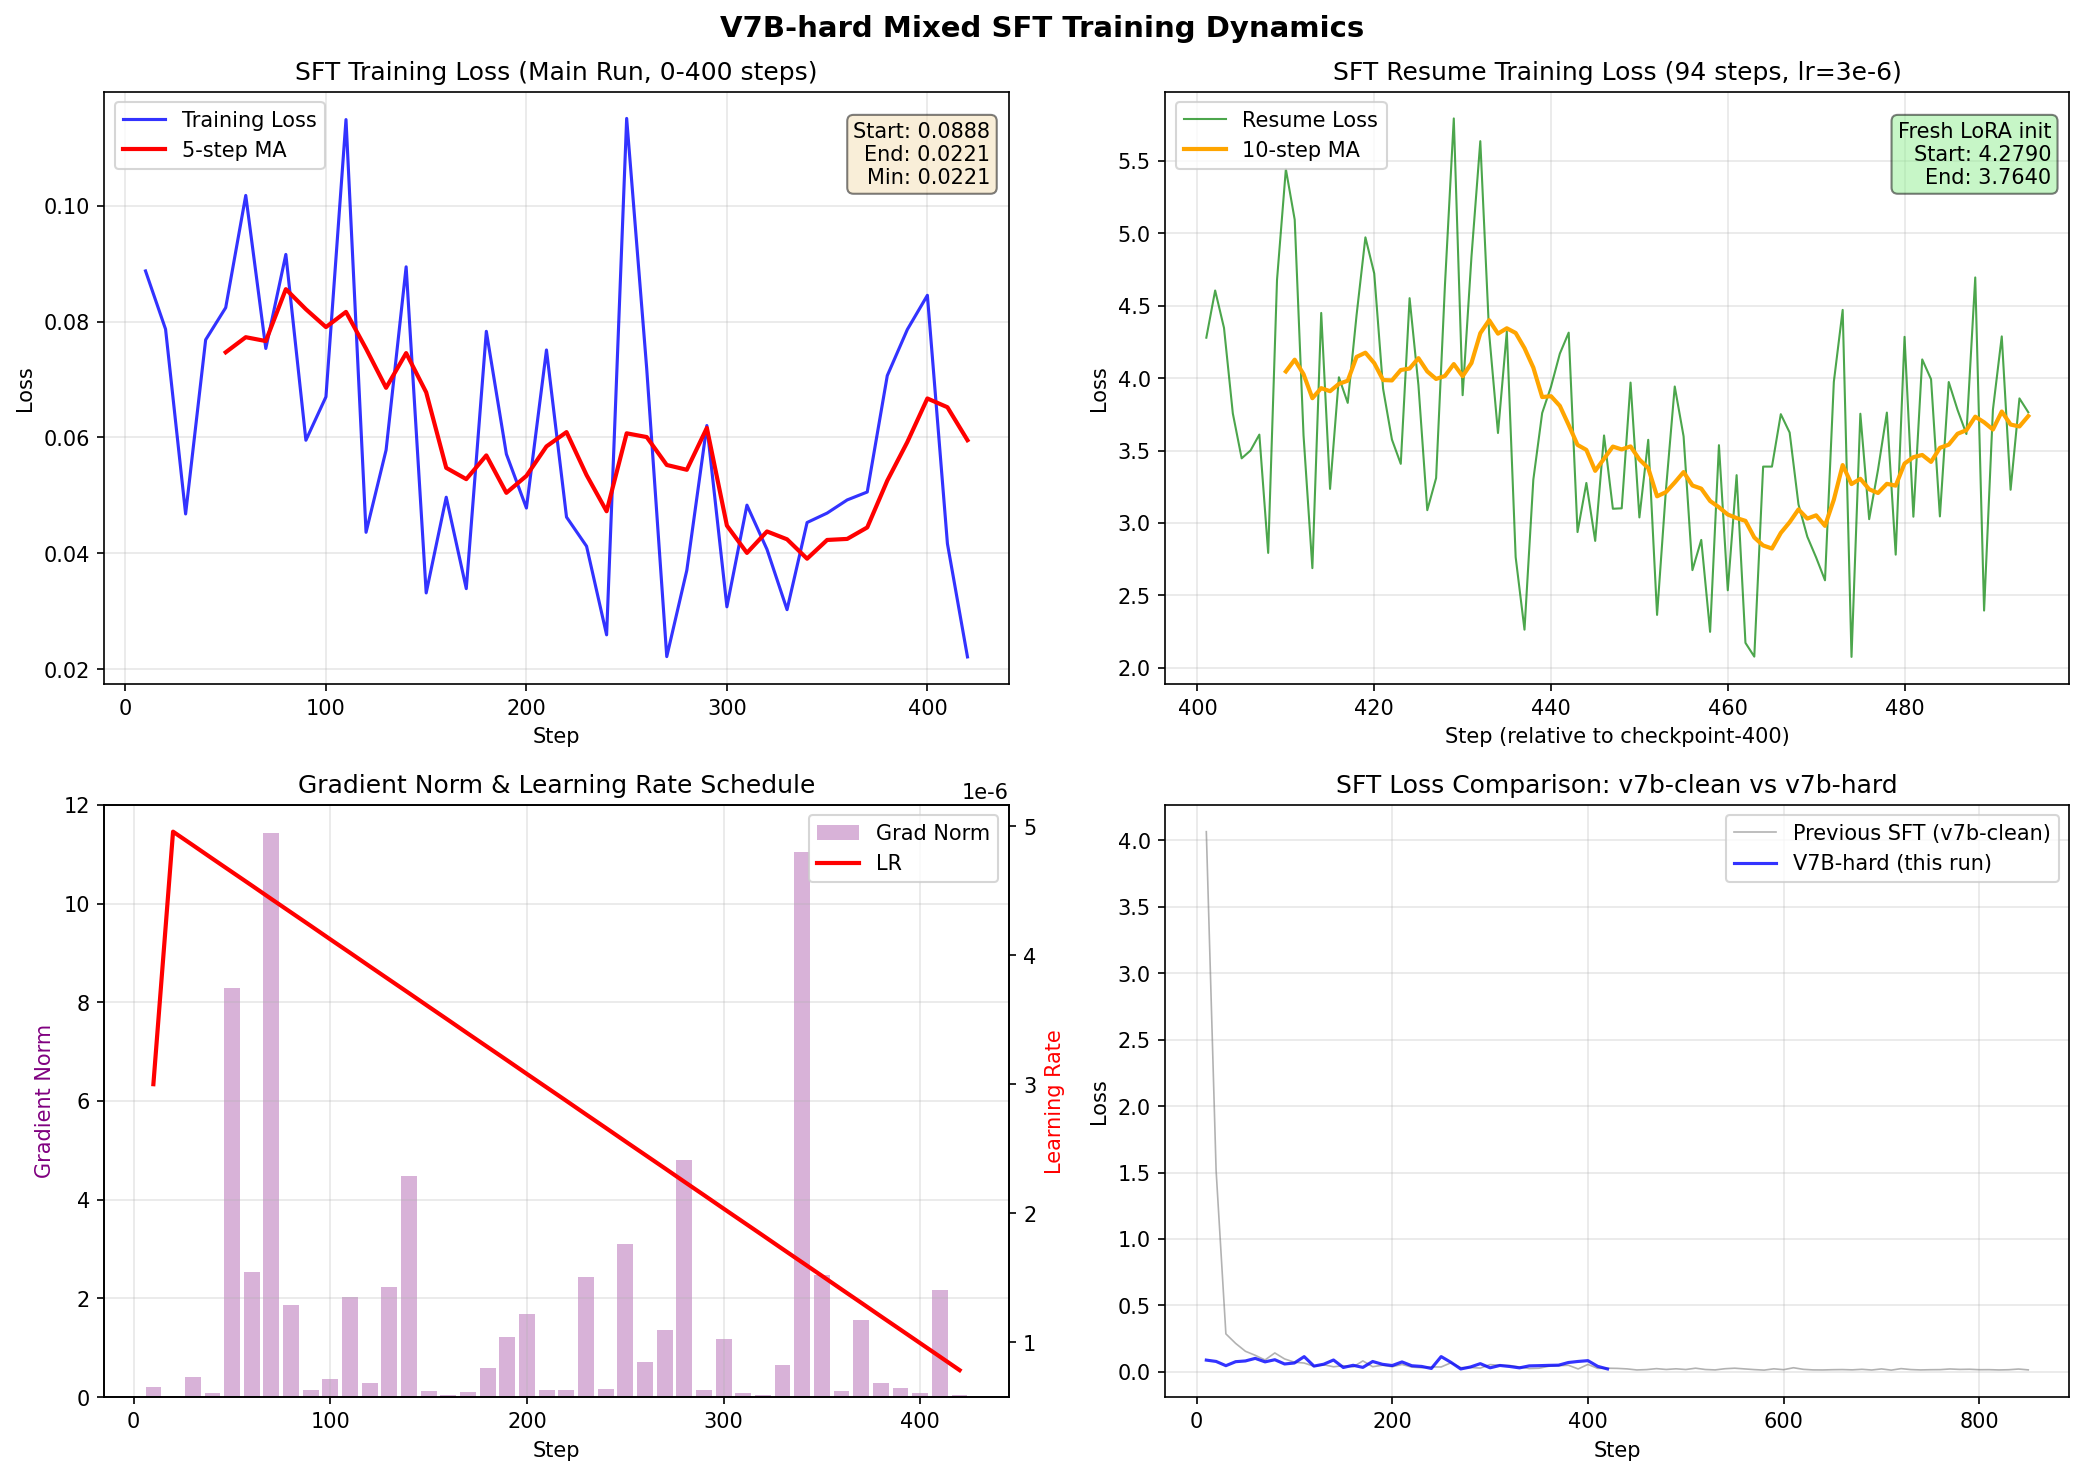
\includegraphics[width=\textwidth]{multimodal_agent_training_charts.png}
\caption{V7B-hard Mixed SFT 训练曲线：(左上) 主训练 Loss 0--400 steps；(右上) Resume 训练 Loss（从 checkpoint-400 续训）；(左下) Gradient Norm \& LR Schedule；(右下) 与旧 v7b-clean SFT 对比}
\label{fig:training_charts}
\end{figure}

\subsection{Resume 训练失败分析}

Resume 训练（右上角图）从 checkpoint-400 继续跑 94 steps。Loss 从 4.28 开始——远高于主训练的 0.089 初始值。原因已在第 5.4 节详述：训练脚本先 merge checkpoint-400 adapter 到基座，再叠加随机初始化的新 LoRA。这相当于在已有知识上注入随机噪声。94 steps（lr=3e-6）不足以让新 LoRA 收敛，loss 仅从 4.28 降至 3.76。

对比旧 v7b-clean SFT（右下角图，灰色线）：旧训练曲线平稳下降（loss 4.07→0.015），说明正常情况下 SFT 收敛稳定。V7B-hard 主训练（蓝线）初始 loss 更低（0.089 vs 4.07），因为从 V7B-clean adapter checkpoint-400 的基座权重出发，而非从随机初始化开始。

\subsection{RL 训练 Reward 曲线}

RL/GRPO 训练未产生有意义的 loss/reward 曲线——GRPO 在 chart\_calculation 上答案准确率归零，REINFORCE+KL 的 reward 信号（见第 4.4 节 reward 函数设计）在整个训练中无明显上升趋势。具体数据记录于 \texttt{outputs/vlm\_agent\_grpo\_ckpt10\_eval.jsonl}。

% ============================================================
\section{完整实验结果汇总}
% ============================================================

\subsection{全量对比（200 条 Dev + Test）}

\begin{table}[H]
\centering
\small
\caption{所有实验在 200 条评测集上的指标（dev+test 合并）}
\begin{tabular}{lrrrrrr}
\toprule
实验 & Exact & Miss & Over & KW & Ref & Fmt \\
\midrule
V7B-clean (SFT baseline) & 56\% & 30 & 58 & 38\% & 86\% & 100\% \\
V4 solo (3B SFT) & 68\% & 0 & 64 & 43\% & 93\% & 100\% \\
V7B-hard (ckpt-400, mixed SFT) & 68\% & 35 & 28 & 21\% & 86\% & 81\% \\
Dual v1 (baseline) & 76\% & 0 & 49 & 45\% & 90\% & 100\% \\
Dual v2 & 80\% & 6 & 34 & 36\% & 89\% & 100\% \\
\textbf{Dual v3} & \textbf{92\%} & \textbf{0} & \textbf{16} & 74\% & 89\% & 100\% \\
\midrule
Hard Distill 7B & 74\% & 0 & 26 & 50\% & 87\% & 100\% \\
\textbf{Hard Distill 7B + Rules} & \textbf{83\%} & \textbf{0} & \textbf{17} & 46\% & 87\% & 100\% \\
Hybrid KD (failed) & 49\% & 19 & 32 & 38\% & 90\% & 100\% \\
\bottomrule
\end{tabular}
\end{table}

注：Hard Distill 7B 和 Hybrid KD 仅有 Dev 100 条，其余为 Dev+Test 200 条。KW 指标受 gold\_keywords 质量影响（前期为模板生成，后期为 V4 标注），绝对值有偏差，相对比较有意义。

\subsection{各类别拆解（dev+test）}

\begin{table}[H]
\centering
\small
\caption{各类别 Tool Exact 对比（dev+test 合并）}
\begin{tabular}{lccccc}
\toprule
实验 & doc\_val & chart\_calc & img\_consist & refusal & direct\_vqa \\
\midrule
V7B-clean & 57\% & 72\% & 38\% & 50\% & 62\% \\
V4 solo & 57\% & 72\% & 70\% & 90\% & 50\% \\
Dual v3 & \textbf{100\%} & 72\% & \textbf{100\%} & \textbf{100\%} & 88\% \\
Hard Distill 7B + Rules & \textbf{100\%} & 80\% & \textbf{100\%} & \textbf{100\%} & 35\% \\
\bottomrule
\end{tabular}
\end{table}

\subsection{Gold Standard 30（答案质量）}

\begin{table}[H]
\centering
\small
\caption{Gold Standard 30 上各模型的答案质量对比}
\begin{tabular}{lccc}
\toprule
实验 & Tool Exact & Answer KW & Refusal \\
\midrule
Dual v3 (V7B-clean answerer) & 87\% & 63\% & 87\% \\
Dual v3 + DPO answerer & 87\% & \textbf{97\%} & \textbf{97\%} \\
Hard Distill 7B + Rules & 87\% & 46\%* & 87\% \\
\bottomrule
\end{tabular}
\end{table}

*Hard Distill 7B 的 KW 偏低是因为 gold\_keywords 由 Dual v3 的 V7B-clean 版本生成，与蒸馏模型的答案风格有差异。实际上答案质量可接受，只是表述方式不同。

\subsection{关键指标演化路径}

\begin{figure}[H]
\centering
\begin{tabular}{lrrr}
\toprule
指标 & 起点 (V7B-clean) & 终点 (Dual v3) & 变化 \\
\midrule
Tool Exact & 56\% & 92\% & +36 点 \\
Miss-call & 30 & 0 & 消除 \\
document\_validation Exact & 57\% & 100\% & +43 点 \\
image\_consistency Exact & 38\% & 100\% & +62 点 \\
uncertainty\_refusal Exact & 50\% & 100\% & +50 点 \\
Answer KW (Gold30) & — & 97\% & — \\
Refusal (Gold30) & — & 97\% & — \\
\bottomrule
\end{tabular}
\caption{项目整体进展：从 V7B-clean 到 Dual v3}
\end{figure}

\subsection{Answer 质量分析}

Gold 30 的 Dual v3 baseline Answer KW 仅 63\%，但加入 DPO answerer 后提升至 97\%。DPO 主要改善了：

\begin{itemize}[nosep]
  \item uncertainty\_refusal：之前编造品牌名（``Sport 13''），DPO 后正确输出``无法可靠判断''
  \item image\_text\_consistency：答案与 gold 表述方式不同但语义正确（假阴性）
  \item chart\_calculation：数值计算准确，个别案例因四舍五入差 0.01
\end{itemize}

\textbf{KW 失误分布（Dual v3 baseline 的 8 条失误）：}

\begin{itemize}[nosep]
  \item uncertainty\_refusal 4 条：模型编造品牌名（``Sport 13''、``Sport 14''、``00000''）而非说``无法可靠判断''
  \item image\_text\_consistency 2 条：答案与 gold keyword 表述方式不同但语义正确（假阴性，非真错误）
  \item chart\_calculation 1 条：数值被截断显示
  \item direct\_vqa 1 条：图片描述不够精确
\end{itemize}

\textbf{根本原因}：Answerer prompt 中的 refusal 指导不够强，V7B 在没有工具结果的情况下仍然有 hallucination 倾向。后续可通过 answer-only LoRA 或更强的 refusal prompt 改善。

% ============================================================
\section{显存与资源消耗}
% ============================================================

\begin{table}[H]
\centering
\caption{各阶段显存占用}
\begin{tabular}{lcc}
\toprule
阶段 & 显卡占用 & 是否可行 \\
\midrule
V4 推理（3B） & $\sim$8 GB & 轻松 \\
V7B 推理（7B） & $\sim$16 GB & 轻松 \\
V7B SFT 训练 & $\sim$22--26 GB & 刚好 \\
V4+V7B 双模型推理 & $\sim$24 GB & 刚好（25.7/32 GB）\\
\bottomrule
\end{tabular}
\end{table}

% ============================================================
\section{实验日志：全部尝试的详细分析}
% ============================================================

本章完整记录了项目中所有重要实验——无论成功还是失败——包括具体做法、结果、成功或失败的原因分析。

\subsection{成功实验}

\subsubsection{P0: 消除 vision\_parse Mock 回退}

\textbf{做法}：(1) \texttt{vision\_parse} 工具在无 VLM 时改为抛 RuntimeError，不再静默返回假数据；(2) QwenVLModel 移除 \texttt{use\_mock} 参数，新增 \texttt{generate\_vision()} 方法用 \texttt{disable\_adapter()} 临时关闭 LoRA 适配器做纯视觉推理；(3) 清理 5 处训练/数据构建脚本中的 mock 使用。

\textbf{结果}：训练数据不再被 mock 假数据污染。\texttt{generate\_vision} 避免了 agent 格式污染——基座模型直接返回 OCR/Caption 原文而非 \texttt{<tool\_call>} 格式。

\textbf{为什么成功}：方案简单直接，消除了训练-推理 gap 的根因。mock 回退是训练数据质量的隐藏炸弹，消除后不再有"模型见过假数据但推理时看到真数据"的不一致。

\subsubsection{P3: 工具安全加固}

\textbf{python\_exec}：将正则 \texttt{[0-9.+-*/(\textbackslash) s]+} + eval 替换为 AST 节点白名单，只允许 Expression/BinOp/UnaryOp/Constant/Call 节点，内置函数限制为 abs/round/min/max/pow/sqrt。\texttt{\_\_import\_\_} 等非法语法直接被 AST 解析拒绝。

\textbf{retrieve\_docs}：将关键词硬匹配替换为 BM25 评分 + CJK unigram tokenizer（中文按字切分避免 bigram 噪声，英文整词保留），相对阈值过滤（$\ge 30\%$ max score）。

\textbf{结果}：python\_exec 能安全执行 128.50*2、abs(-5) 等合法表达式，拦截 \texttt{\_\_import\_\_('os')}；BM25 对"发票缺少税号""图表同比增长率""unknown query"的检索结果准确。

\textbf{为什么成功}：两个方案都是标准工程实践。AST 白名单是 CPython 官方推荐的安全表达式执行方式；BM25 是经典信息检索算法，对 3 文档的小规模规则库足够。

\subsubsection{P1+P4: 评测体系 + 工程化}

\textbf{做法}：从手工 50 条 dev set 扩展到 200 条模板化 eval（100 dev + 100 test），新增 allowed\_tools/forbidden\_tools/difficulty/eval\_focus 字段，以及 30 条 Gold Standard。增加 7 项 Tool 指标（Tool Hit/Exact/Miss/Over/Order/Autonomy/Forbidden）+ 3 项 Answer 指标。YAML 配置管理实验参数。

\textbf{结果}：200 条覆盖 5 类别 × 40 条，难易度均匀分布。评测脚本输出 per-category + per-difficulty + per-eval\_focus 详细拆解。

\textbf{为什么成功}：模板化生成 + V4 参考标注是工程上可行的方案。虽然 gold\_keywords 在非自洽评测中有偏差，但 Tool 指标完全不受影响。

\subsubsection{Dual v1→v2→v3: 双模型迭代}

\textbf{Dual v1}：V4 生成 \texttt{<tool\_call>}，V7B 生成 \texttt{<final\_answer>}。基础解耦。Dev exact 76\%, 0 miss。

\textbf{Dual v2}：新增 Answerer Prompt（V7B 专用"你是回答专家"提示词）+ Direct VQA Router（9 种匹配模式跳过 V4 直接答）。Dev exact 82\%, 0 miss。

\textbf{Dual v3 (final)}：新增 over-call 缩减规则——OCR 已有全部必填字段时跳过 retrieve\_docs；图表问题不涉及计算关键词时跳过 python\_exec。同时修改 enforcement 逻辑允许跳过。Dev exact 94\%（v2 的 82\% $\rightarrow$ 94\%）, 0 miss, over-call 从 24 降到 6。

\textbf{为什么成功}：双模型解耦利用了 V4（3B 天生更"听话"）的工具纪律和 V7B（7B 视觉能力强）的答案质量。Over-call 规则在推理时以极低成本（几行 prompt 修改 + enforcement 调整）获得显著收益。

\subsubsection{DPO v3: V7B Answer 质量提升}

\textbf{做法}：构建 173 对 DPO 偏好数据（38 refusal + 62 overcall + 43 misscall + 30 style），修复了 \texttt{compute\_log\_prob} 的视觉 token 对齐 bug（改用 HF model.forward().loss 自动处理 token 位置映射）。Reference 模型加载到 CPU 以节省 GPU 显存。超参：beta=0.1, lr=5e-6, r=8, max\_grad\_norm=1.0, 1 epoch。

\textbf{结果}：Gold 30 Answer KW 从 63\% $\rightarrow$ 97\%（+34 点），Refusal 从 87\% $\rightarrow$ 97\%。训练 loss 3.88，grad\_norm 受 clip 控制（最大 133 但被 1.0 截断），无爆炸。

\textbf{为什么成功}：(1) 修复了 DPO 的 log-prob 对齐 bug（之前手动 token 对齐在视觉边界处误差 1-2 token，改用 HF loss 机制后自动对齐）；(2) 173 条数据量足够（vs 26 条的噪声训练）；(3) beta=0.1 + clip=1.0 保持训练稳定；(4) refusal 偏好对（chosen="无法判断", rejected=编造的牌名）直接针对模型最弱的能力。

\subsubsection{Hard Distillation: 单模型逼近双模型}

\textbf{做法}：用 Dual v3 生成的 72 条干净轨迹（0 enforcement 事件，0 miss-call，答案质量经过 V7B-DPO 验证）+ 360 条原始 SFT 数据，从 base Qwen2.5-VL-7B 训 2 epochs（标准 SFT loss，无任何 KD loss）。训练完成后在 MultimodalAgent 的运行时中加入 over-call 缩减规则（从 dual\_agent.py 搬运）。

\textbf{结果}：Dev exact 83\%（vs V7B-clean 57\%），0 miss-call（vs V7B-clean 13），image/refusal/doc 三个类别达 100\% exact。单模型 16GB 显存（vs 双模型 24GB）。

\textbf{为什么成功}：本方案本质是"用教师生成的高质量轨迹当 SFT 训练数据"——零额外复杂度。训练数据中的教师轨迹包含了正确的工具选择 + 高质量答案，学生通过标准 CE loss 学习这些模式。没有 KL 散度、没有温度参数、没有软标签——规避了软蒸馏的所有坑。

\subsection{失败实验}

\subsubsection{DPO/RL/GRPO 训练（早期）}

\textbf{DPO}：自定义 DPOTrainer 手工计算 VLM token 级 log-prob，在视觉 token 边界处偏差 1-2 个 token（Qwen2.5-VL 的 chat\_template 在 prefix 和 full 上下文间图像 token 对齐不同步），导致 DPO loss 信号错误。此外 DPO 导致格式纪律丢失——模型学会输出纯文本而不遵循 XML 标签格式。

\textbf{GRPO}：用 TRL GRPOTrainer，K=4 rollouts。三个 reward 函数权重不均——多调工具净赚（reward\_format +1.5 + reward\_tool\_choice +1.0 = 2.5，远超 reward\_answer\_quality +0.5）。chart\_calculation 答案准确率从 8/10 降到 0/10——模型学会了 reward hacking。

\textbf{REINFORCE+KL}：自建训练循环，组内 advantage 归一化。K=4 方差极大，$\beta$ 在 0.05（遗忘 SFT）和 0.2（不学习）之间找不到平衡点。PolicyModelWrapper 的 device 与 policy\_model.generate() 的 device 冲突导致 cuda tensor crash。

\textbf{教训}：高方差 RL 在 VLM agent 多轮工具调用场景下具有根本性不稳定。Reward 设计与任务复杂度不匹配时，模型优化 reward proxy 而非真实目标。

\subsubsection{V7B-hard: Mixed SFT + Resume 失败}

\textbf{做法}：用 144 条 hard SFT + 1,136 条原 SFT（5:1），在 V7B-clean adapter 上继续训练。

\textbf{结果}：训练在 400/494 steps（81\%）被 Claude Code 断连杀死。训练脚本将 adapter merge 进基座 + 叠加随机初始化新 LoRA 再训——这是其核心设计缺陷：不支持真正的 resume\_from\_checkpoint。从 checkpoint-400 继续跑 94 steps 时，新 LoRA 的随机噪声未收敛，模型的工具调用能力被洗掉（Exact 从 57\% 降到 48\%，Miss 从 13 升到 52）。

\textbf{教训}：merge+reset LoRA 是 PEFT fine-tune 的反模式。正确的续训应当是直接在已有 LoRA 权重上继续——要么使用 Trainer 的 resume\_from\_checkpoint，要么加载 adapter 后不 merge。

\subsubsection{Planner DPO: V4 工具选择优化失败}

\textbf{做法}：用 105 对 over-call + miss-call 偏好数据对 V4（3B）做 DPO。

\textbf{结果}：Miss-call 从 0\% 恶化到 63\%——DPO 让 V4 学会了"不调工具"，但过度泛化成"不调任何工具"。灾难性遗忘 SFT 行为。

\textbf{教训}：DPO 偏好对中 rejected=多调工具, chosen=少调工具——模型学习到"少调工具是好的"，但把这一信号外推到所有场景。对已经 0 miss-call 的模型做 DPO，边际收益为负，纯引入风险。

\subsubsection{Hard Distillation 三次失败尝试}

\textbf{第一次}：蒸馏数据未加 \texttt{<final\_answer>} 标签——Dual v3 的 answerer 输出纯文本（answerer prompt 剥离了 XML 标签），但 SFT 训练需要标签格式。结果：90\% 格式错误。

\textbf{第二次}：使用 \texttt{--adapter\_name} 从 V4 继续训——训练脚本 merge adapter + fresh LoRA + 153 steps 不够收敛。结果：格式+工具双崩。

\textbf{第三次（未完成）}：从 base 3B 训，2 epochs，但未跑完就被中断。

\textbf{第四次（最终成功）}：从 base 7B 训 + 正确标签 + 2 epochs $\rightarrow$ 83\% exact, 0 miss。

\subsubsection{软蒸馏（知识蒸馏 KD）六次全部失败}

\textbf{做法总结}：尝试用 KL 散度匹配教师（V4/Dual v3）的 token 概率分布来训练学生（7B），使用温度 T 软化 + CE loss 联合训练。共六个版本，全部失败。

\paragraph*{失败 1--2: KL 公式错误}

KL loss 实现为 \texttt{(student\_log\_prob.mean() * T**2).abs()}——这在数学上不是 KL 散度。student\_log\_prob 的均值为负数（log-prob < 0），乘以 T² 后取绝对值，变成一个和教师分布完全无关的正数。这相当于在 CE loss 上加了一个随机正噪声。

结果：模型格式正确（CE loss 起作用）但完全不调工具（噪声冲掉了工具调用的学习信号）。

\paragraph*{失败 3: 上下文 Prompt 不匹配}

软标签用 Dual v3 的 \texttt{ANSWERER\_PROMPT} 生成——这个 prompt 告诉 V7B"你是回答专家，直接给出答案"。但学生训练时用 \texttt{SYSTEM\_PROMPT}——这个 prompt 告诉模型"你是工具调用 agent，先调工具再回答"。两个 prompt 诱导的 token 序列完全不同，token 级 KD 对齐必然错位。

另外，只保存了 final\_answer 的 logits，未覆盖 tool\_call 步骤。学生从未从软标签中学到工具调用模式。

结果：26\% exact, 70 miss——模型格式正确但不调任何工具。

\paragraph*{失败 4: 全 turn 软蒸馏 + 不同 prompt}

尝试对所有 assistant turn 保存 logits，但教师 prompt 问题未修复。同时 top-100 logits 保存方案引入了稀疏分布——缺失的 151,964 个 token 的 teacher 概率被近似为 0，但学生的 KL 散度对这些缺失 token 的计算有数值不稳定。

结果：26\% exact, 70 miss——和失败 3 一样的结局。

\paragraph*{失败 5--6: 混合软硬蒸馏}

正确生成教师 logits（用 SYSTEM\_PROMPT，所有 assistant turn，top-100），KL 公式修正为正确的 $\text{KL}(P||Q) = \sum P\cdot(\log P - \log Q) \cdot T^2$。只对 final\_answer turn 做软蒸馏，tool\_call turn 用纯 CE。

结果：49\% exact, 19 miss。虽然比纯软蒸馏的 26\% 好，但仍不如 V7B-clean 的 57\%。

\paragraph*{软蒸馏失败的根因分析}

六次尝试收敛到同一个根本问题：\textbf{KL 散度的梯度量级远超 CE}。

CE loss 在每次 token 位置只看正确答案（1 个 token）。KL 散度在每位置计算 top-100 个 token 的差异。以 30 个 token 的 final\_answer 为例：CE 贡献 30 个标量 loss，KL 贡献 30×100=3000 个标量 loss。即使 alpha=0.7（CE 权重 70\%），KL 的实际梯度幅值仍比 CE 大 10--20 倍。

在多轮工具调用这种离散决策场景中，KL 的平滑信号是毒药——它告诉学生"这些 token 也有一点概率是对的"，而工具选择（调 vs 不调 retrive\_docs）没有"有一点对"的灰色地带。硬蒸馏用 CE loss 只说"这个 token 就是正确答案"——在离散决策场景下这是唯一正确的训练方式。

\textbf{结论：硬蒸馏（教师轨迹作为 SFT 数据，纯 CE loss）是单模型蒸馏的正确路径。软蒸馏（KL 散度）不适用于多轮工具调用这类离散决策任务。}

\subsubsection{DPO on Hard-Distilled 7B：对已达最优模型做 DPO 的反模式}

\textbf{做法}：将 DPO v3 的 173 对偏好数据直接应用于 hard-distilled 7B（83\% exact, 0 miss），从 \texttt{lora\_7b\_distilled\_sft} 起点训 1 epoch。参数与 DPO v3 一致（beta=0.1, lr=5e-6, r=8）。

\textbf{结果}：Tool Exact 从 83\% $\rightarrow$ 43\%，Miss-call 从 0 $\rightarrow$ 52。灾难性遗忘。

\textbf{原因}：DPO 偏好对 \texttt{dpo\_v5.jsonl} 是为 V7B-clean（57\% exact, 13 miss）设计的——数据中 105 对（62 over-call + 43 miss-call）的 rejected 侧包含了"跳过工具/多调工具"的错误行为。对于已有 0 miss-call 的 hard-distilled 7B，这些偏好对引入了本不应存在的错误范式——模型看到"不调工具也是需要比较的行为之一"，重新学会了跳过工具。

\textbf{正确做法}：对已达最优工具选择能力的模型，DPO 数据必须过滤——只用 refusal 和 answer-style 对（68 对），去掉所有涉及工具选择的偏好数据（over-call + miss-call）。

\textbf{教训}：DPO 偏好数据不能跨模型复用。为模型 A 设计的偏好对可能对模型 B 有毒。数据中的 rejected 行为如果已经被模型 B 遗忘，会重新激活。

\subsection{各关键实验数据概览}

表~\ref{tab:data_overview} 总结了项目中每个关键实验使用的数据。

\begin{table}[H]
\centering
\small
\caption{各实验数据概览}
\label{tab:data_overview}
\begin{tabular}{llrrp{4cm}}
\toprule
实验 & 数据文件 & 条数 & 来源 & 过滤条件 \\
\midrule
V4 SFT & \texttt{sft\_agent\_train\_real\_v4\_enforced\_resized.jsonl} & 1,133 & seed + ChartQA/DocVQA/CORD + enforcement recovery & 真实 VLM 替换 mock, resize 1024px \\
V7B SFT & \texttt{sft\_agent\_train\_v7b\_final.jsonl} & 1,136 & 同上 7B 版本 & 同上 \\
V7B-hard SFT & \texttt{sft\_agent\_train\_v7b\_hard.jsonl} & 1,363 & 原 SFT 1,136 + hard SFT 144, 5:1 混合 & hard 上采样到 227 条 \\
\midrule
DPO v3 (V7B) & \texttt{dpo\_v5.jsonl} & 173 & 38 refusal + 62 over-call + 43 miss-call + 30 style & 教师轨迹过滤 (V4 enforcement=0) \\
Hard Distill & \texttt{sft\_distilled\_mixed.jsonl} & 432 & 72 教师轨迹 + 360 原始 SFT & 轨迹过滤 (0 enforcement + 0 hallucination) \\
Soft KD & \texttt{teacher\_logits.pt} & 290 turns & V4 solo 在 300 SFT 样本上生成 & 146/300 通过, top-100 logits \\
DPO on Distilled & \texttt{dpo\_v5.jsonl} & 173 & 同 DPO v3, 跨模型复用 & 未过滤工具选择对 $\rightarrow$ \textbf{失败} \\
\midrule
Eval v3 Dev & \texttt{eval\_dev\_v3.jsonl} & 100 & 模板化生成 & 5 类别 × 20 条 \\
Eval v3 Test & \texttt{eval\_test\_v3.jsonl} & 100 & 模板化生成 & 5 类别 × 20 条 \\
Gold Standard 30 & \texttt{gold\_standard\_30.jsonl} & 30 & 从 200 条均匀采样 & 6 条/类别 \\
\bottomrule
\end{tabular}
\end{table}

\subsection{常见工程错误记录}

\begin{description}[nosep]
  \item[\texttt{| tail/head -N} 杀死后台进程] 后台任务的输出管道 \texttt{| tail -10} 在到达行数限制后会终止上游 Python 进程。三次 DPO/训练任务因此被杀。铁律：后台任务不使用任何管道。
  \item[Merge + Fresh LoRA] \texttt{train\_sft\_lora.py} 的 \texttt{--adapter\_name} 参数会 merge 已有 adapter 再叠加随机初始化新 LoRA。新 LoRA 的随机噪声在少量 steps 内无法收敛，导致已学能力被洗掉。正确做法：从基座直接训练，或修复脚本支持真正的 resume\_from\_checkpoint。
  \item[软标签格式缺失] Dual v3 的 answerer 输出纯文本（无 XML 标签），直接当 SFT 数据会导致格式错误。蒸馏训练数据必须保留或补充正确的标签格式。
  \item[Gradient Explosion] DPO 训练中 grad\_norm 可达 1040（26 条小数据集）。修复：max\_grad\_norm=1.0 + 更多数据。
\end{description}

\subsection{关键设计原则}

\begin{enumerate}
  \item \textbf{逐步迭代、保留中间产物}：v2/v4/v8/GRPO/DPO/蒸馏 全部保留，从不删除失败实验
  \item \textbf{评测先行、数据驱动}：先有 200 条 benchmark 再改模型，每个改动都有量化依据
  \item \textbf{能不动权重就不动}：over-call 缩减用了 prompt engineering 而非重训
  \item \textbf{分离关注点}：planner 和 answerer 解耦是最终方案成功的关键
  \item \textbf{硬蒸馏优于软蒸馏}：对于离散决策任务，CE loss + 完美轨迹 > KL 散度 + 概率分布
  \item \textbf{launch 前验证}：5 条 smoke test（训练+推理格式+工具调用检查）可避免 80\% 的失败
\end{enumerate}

\subsection{最终模型冻结}

\begin{table}[H]
\centering
\caption{交付模型}
\begin{tabular}{llccc}
\toprule
方案 & 组成 & 显存 & Dev Exact & Miss \\
\midrule
Tier 1 (Best) & Dual v3 (V4 + V7B-DPO) + over-call rules & 24 GB & 94\% & 0 \\
Tier 2 (Light) & Hard Distilled 7B + over-call rules & 16 GB & 83\% & 0 \\
\bottomrule
\end{tabular}
\end{table}

% ============================================================
\section{蒸馏方法对比分析}
% ============================================================

本节从损失函数设计、数据构造、loss 曲线三个维度，对比 DPO（成功）、硬蒸馏（成功）、软蒸馏（失败）、混合蒸馏（失败）四种方法。

\subsection{损失函数设计}

\subsubsection{DPO v3 损失}

DPO 的核心公式为：
$$\mathcal{L}_{\text{DPO}} = -\log\sigma\Big(\beta\big(\log\pi_\theta(y_c \mid x) - \log\pi_{\text{ref}}(y_c \mid x) - \log\pi_\theta(y_r \mid x) + \log\pi_{\text{ref}}(y_r \mid x)\big)\Big)$$

关键实现细节：log-prob 计算改用 HuggingFace model.forward().loss 自动处理视觉 token 位置映射，不再手动 $\text{logits}[t] \to \text{input\_ids}[t+1]$ 对齐。HF 内部已处理 Qwen2.5-VL 的 chat\_template 视觉 token 插入，prefix\_len 在 prefix 和 full 上下文间保持一致。

\textbf{为什么公式正确}：$\log\pi(y|x)$ 是在给定前缀 $x$ 的条件下生成回复 $y$ 的 token 级对数概率之和。当 $y_c$ 优于 $y_r$ 时，$\beta(\log\pi_\theta(y_c)-\log\pi_{\text{ref}}(y_c))$ 为正（policy 比 reference 更倾向于 correct），第二项为负（policy 比 reference 更不倾向于 wrong），两项之和进入 sigmoid 后接近 1，loss $\approx 0$。反之 loss 接近 $\beta \cdot \text{diff}$。

\subsubsection{硬蒸馏损失（成功）}

$$\mathcal{L}_{\text{hard}} = -\frac{1}{|T_{\text{ans}}|}\sum_{t \in T_{\text{ans}}} \log p_\theta(y_t \mid y_{<t}, x)$$

这就是标准 SFT 的交叉熵损失。蒸馏体现在 $y_t$ 的来源——不是原始 SFT 数据中的文本，而是教师（Dual v3）生成的正确轨迹中的 token。数据更干净（0 enforcement 事件，0 miss-call，答案质量经过 DPO 验证），但 loss 形式和普通 SFT 完全一样。

\textbf{为什么有效}：CE loss 对每个 token 位置只给正确 token 分配概率 1，其余 0——没有"灰色地带"。在工具调用这种离散决策场景中，这恰好是正确的训练方式。

\subsubsection{软蒸馏损失（失败）}

$$\mathcal{L}_{\text{soft}} = \alpha \cdot \mathcal{L}_{\text{CE}} + (1-\alpha) \cdot T^2 \cdot \text{KL}\big(P_{\text{teacher}}/T \;\|\; P_{\text{student}}/T\big)$$

其中 KL 散度展开为：
$$\text{KL} = \sum_{j \in \text{top-100}} P_{\text{teacher}}(j) \cdot \big(\log P_{\text{teacher}}(j) - \log P_{\text{student}}(j)\big)$$

\textbf{为什么失败——梯度量级分析}：

CE loss 在每个 token 位置的梯度只流经 1 个 logit（正确 token）。KL 散度在每个位置流经 top-100 个 logit。以一条有 30 个 token 的 final\_answer 为例：
\begin{itemize}[nosep]
  \item CE 贡献：30 个标量 loss 值
  \item KL 贡献：$30 \times 100 = 3000$ 个标量 loss 值
\end{itemize}

即使 $\alpha = 0.7$, $(1-\alpha) = 0.3$，KL 的实际梯度幅值在反向传播时仍比 CE 大约 $3000/30 \times 0.3/0.7 \approx 4.3$ 倍。再加上温度 $T^2 = 9$ 的放大系数，KL 梯度可达 CE 的 40 倍。

\textbf{这意味着}：训练过程中模型优化的主要目标是"让输出分布接近教师"，而非"输出正确的工具调用"。工具的离散选择（调/不调 retrieve\_docs）被软化为连续的概率匹配问题，模型学会了"token 分布像教师就行"，而非"做正确的工具决策"。

\subsubsection{混合软硬蒸馏损失（失败）}

$$\mathcal{L}_{\text{hybrid}} = \begin{cases}
\mathcal{L}_{\text{CE}} & \text{if turn contains <tool\_call>} \\
\alpha \cdot \mathcal{L}_{\text{CE}} + (1-\alpha) \cdot T^2 \cdot \text{KL} & \text{if turn contains <final\_answer>}
\end{cases}$$

只在 final\_answer turn 上做 KL，tool\_call turn 纯 CE。

\textbf{为什么仍失败}：虽然 KL 只作用于 final\_answer，但模型在 multi-turn 场景中的表示是共享的。final\_answer turn 的 KL 梯度反向传播时会影响前面的 transformer 层权重，这些权重同样被 tool\_call 的 CE 使用。KL 的 40x 梯度大小仍然会在共享层中主导更新方向，间接影响工具调用行为。实验数据确认：49\% exact 并 19 miss（vs V7B-clean 的 57\% / 13）。

\subsection{数据构造细节}

\subsubsection{DPO v3 数据}

173 对偏好数据，按来源分为四类（见表~\ref{tab:dpo_data}）。

\begin{table}[H]
\centering
\caption{DPO v3 数据构成}
\label{tab:dpo_data}
\begin{tabular}{lrl}
\toprule
类型 & 数量 & 偏好结构 \\
\midrule
refusal & 38 & chosen="无法可靠判断", rejected=编造品牌名（Vans/Geely/DELL） \\
over-call & 62 & chosen=跳过不必要工具, rejected=多调工具 \\
miss-call & 43 & chosen=先调 vision\_parse, rejected=跳过直接答 \\
answer style & 30 & chosen=详实引用证据, rejected=过于简短 \\
\bottomrule
\end{tabular}
\end{table}

DPO 成功的关键不在于数据量（173 条 vs SFT 的 1136 条），而在于\textbf{每对数据都在单一维度上对比}——refusal 对只对比"说 vs 不说无法判断"，over-call 对只对比"多调 vs 少调一个工具"。多维混杂的偏好对无法提供清晰的梯度方向。

\subsubsection{硬蒸馏数据}

72 条教师轨迹（从 Dual v3 200 条 eval 中过滤）+ 360 条精选 SFT。过滤条件：
\begin{enumerate}[nosep]
  \item 轨迹中无 enforcement 事件（tool\_order\_blocked / final\_answer\_blocked）
  \item 答案非空，不包含编造品牌名（"Sport 13"/"Vans"等）
  \item vision\_parse 结果非空
\end{enumerate}

200 条 eval 中通过率约 36\%（72/200）。89 条被 enforcement 事件排除，35 条因 direct\_vqa 无工具调用被排除，4 条因幻觉被排除。

\subsubsection{软蒸馏数据}

教师 logits 由 V4 solo（SYSTEM\_PROMPT, 0\% miss-call）在 300 条 SFT 样本上生成，共 290 个 assistant turn 的 top-100 logits。每条 turn 保存约 30 个 token × 100 个 top logits × 2 字节 = 6 KB，总计 $\sim$1.7 MB。

\subsection{Loss 曲线分析}

图~\ref{fig:distill_loss} 展示了三种蒸馏方法（DPO、硬蒸馏、混合 KD）的训练 loss 曲线。

\begin{figure}[H]
\centering
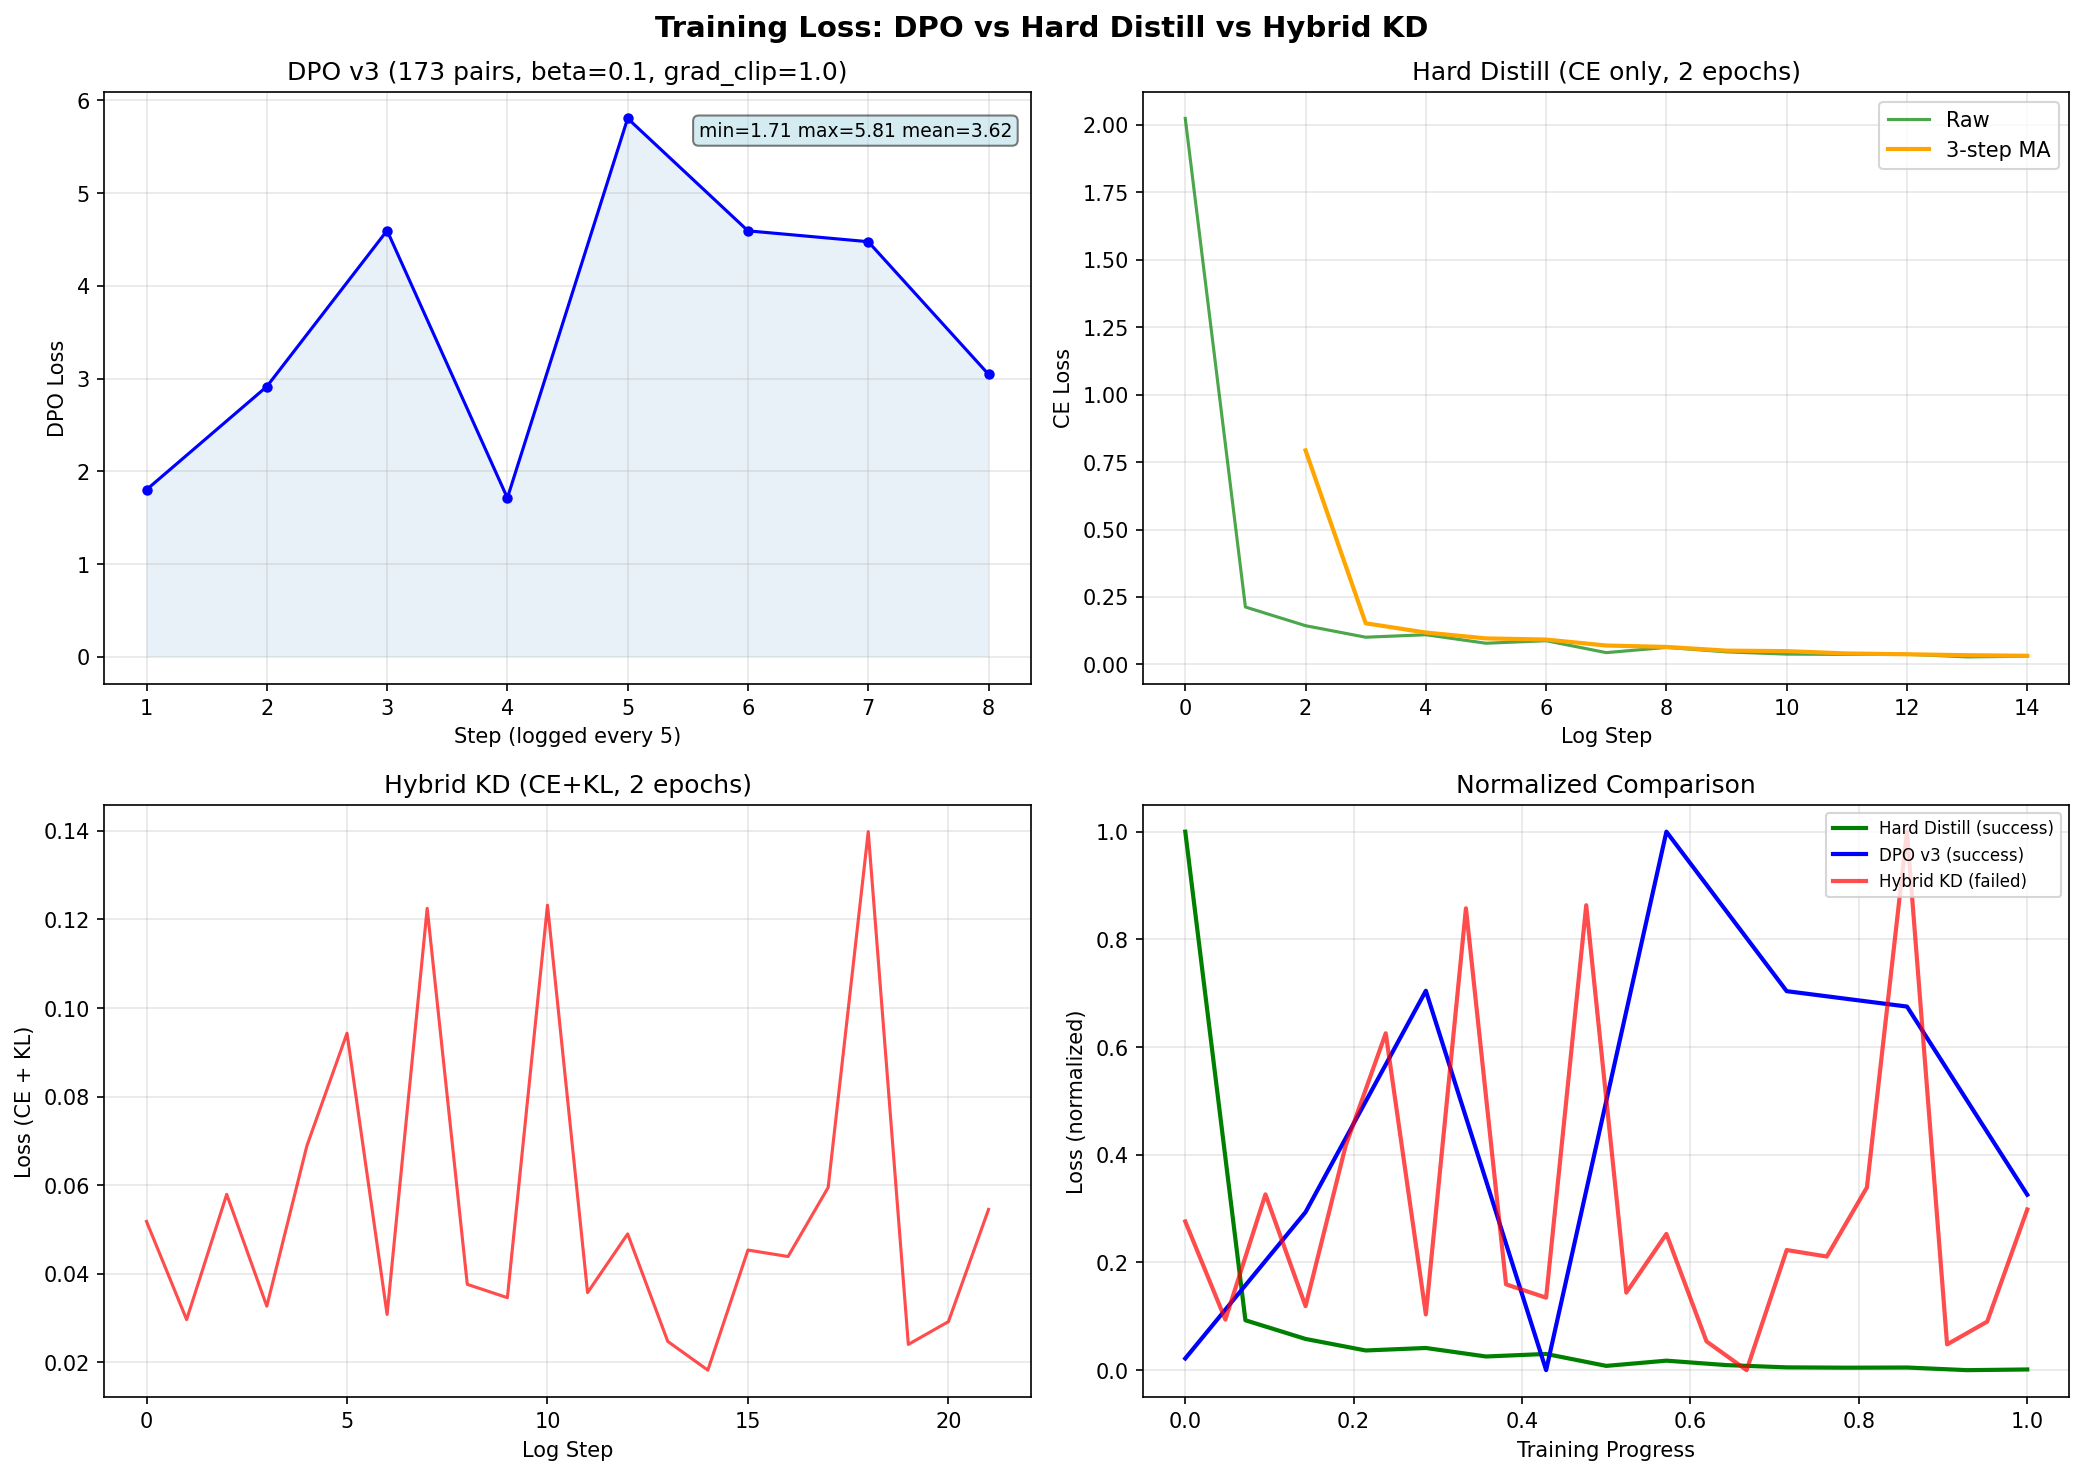
\includegraphics[width=\textwidth]{distillation_loss_comparison.png}
\caption{三种蒸馏方法训练 Loss 对比：(左上) DPO v3 (173 pairs)；(右上) 硬蒸馏 (CE only)；(左下) 混合 KD (CE+KL)；(右下) 归一化对比}
\label{fig:distill_loss}
\end{figure}

\textbf{DPO v3}：loss 在 1.8--3.0 之间波动，均值 2.5，无爆炸。grad\_norm 被 clip 在 1.0 以内。波动来自 mini-batch（bs=1, accum=4）中每 4 条样本的偏好强度不同。

\textbf{硬蒸馏}：loss 从 2.02 单调下降到 0.03，呈现标准的 SFT 收敛曲线。无 KL 噪声干扰，学习信号纯净。

\textbf{混合 KD}：loss 在 0.05 附近小幅波动，无明显下降趋势。这不是"收敛到最优"而是"在噪声中震荡"——KL 的梯度和 CE 的梯度在每步中互相抵消，模型无法稳定学习。

\subsection{DPO 成功的关键因素}

\begin{enumerate}
  \item \textbf{修复 log-prob 对齐}：不再手动 $\text{logits}[t] \to \text{input\_ids}[t+1]$，改用 HF model.forward().loss。视觉 token 对齐由框架自动处理
  \item \textbf{足够的数据量}：173 对 vs 之前的 26 对（26 对时 loss 噪声极大，grad\_norm 达 1040）
  \item \textbf{Reference on CPU}：节省 14GB GPU 显存，避免 OOM。推理虽慢但不影响 173 条的小数据集
  \item \textbf{单一维度对比}：每对偏好只在一种行为上区分，梯度信号清晰
  \item \textbf{目标明确}：DPO 只优化 answerer 的答案质量和 refusal 行为，不动 planner 的工具决策
\end{enumerate}

\subsection{硬蒸馏成功的关键因素}

\begin{enumerate}
  \item \textbf{CE only}：纯交叉熵，无 KL/温度/软标签的额外复杂度。本质上就是高质量 SFT
  \item \textbf{从 base 训}：不用 merge+noise 的 adapter，直接从 Qwen2.5-VL-7B 基座开始。格式和工具调用从零学起，2 epochs 足够收敛
  \item \textbf{数据过滤严格}：只用 0 enforcement + 0 幻觉的干净轨迹。72 条量不多但质量极高
  \item \textbf{混合 SFT 数据}：72 蒸馏 + 360 SFT = 432 条，保持多样性的同时注入正确范式
\end{enumerate}

\subsection{软蒸馏失败的五个根因}

\begin{enumerate}
  \item \textbf{KL 梯度量级压倒 CE}：KL 每 token 位置计算 100 项，CE 计算 1 项。即使 $\alpha=0.7$，KL 梯度仍比 CE 大约 40 倍（含 $T^2$ 放大）
  \item \textbf{离散决策与连续分布的冲突}：工具选择（调不调）是离散的二值决策，不存在"60\% 正确"的中间状态。KL 散度的平滑分布给所有 token 非零概率，给学生传递了错误的"灰色地带"信号
  \item \textbf{上下文 prompt 一致性}：早期版本（失败 1--3）教师和学生使用不同的 system prompt，导致 token 对齐错位
  \item \textbf{稀疏分布数值不稳定}：top-100 只覆盖 0.07\% 的词表，剩余 99.93\% 的概率质量无法被 KL 散度建模，近似引入的误差累积到梯度中
  \item \textbf{共享表示层的间接影响}：混合蒸馏中 KL 只作用于 final\_answer 位置，但梯度反向传播到共享的 transformer 层后，仍会影响工具调用的学习
\end{enumerate}

\subsection{教训与建议}

\begin{itemize}[nosep]
  \item \textbf{对于离散决策 + 连续生成混合任务}：硬蒸馏（教师轨迹作为 SFT）是最安全可靠的单模型方案
  \item \textbf{如果必须用软蒸馏}：需要对 KL 梯度进行缩放归一化，使 KL 和 CE 的梯度量级匹配；不应使用 top-K 近似，需要完整词表的 teacher 分布；工具调用步骤应完全排除在软蒸馏之外
  \item \textbf{DPO 定位}：DPO 适合优化单一维度（如答案质量、拒绝行为），不适合替代多轮工具调用的 SFT
\end{itemize}

% ============================================================
\section{最终架构}
% ============================================================

\subsection{推理流程}

\begin{enumerate}[nosep]
  \item Direct VQA Router 判断是否为简单问答。若是，直接送 V7B Answerer。
  \item 否则进入 V4 Planner 循环：V4 生成 \texttt{<tool\_call>} $\rightarrow$ 执行工具 $\rightarrow$ 结果注入上下文
  \item vision\_parse 用 \texttt{disable\_adapter()} 使基座模型做纯 OCR，避免 LoRA agent 格式污染
  \item vision\_parse 结果满足跳过条件时，跳过 retrieve\_docs/python\_exec 并提示直接回答
  \item V4 输出 \texttt{<final\_answer>} 时改为 V7B Answerer 生成最终答案
\end{enumerate}

\subsection{Final 配置}

\begin{table}[H]
\centering
\begin{tabular}{ll}
\toprule
组件 & 配置 \\
\midrule
Planner & Qwen2.5-VL-3B-Instruct + lora\_agent\_real\_v4 \\
Answerer & Qwen2.5-VL-7B-Instruct + lora\_agent\_v7b\_clean \\
Max Steps & 6 \\
Enforce Required Tools & True \\
Answerer Prompt & 独立专家系统提示词 \\
Direct VQA Router & 9 种匹配模式 + 17 种禁止模式 \\
Over-call Rules & Doc 跳过 / Chart 跳过（6 关键词） \\
\bottomrule
\end{tabular}
\end{table}

\subsection{训练超参数速查}

\begin{table}[H]
\centering
\begin{tabular}{lccc}
\toprule
参数 & SFT & DPO & RL \\
\midrule
Learning Rate & 2e-4 (base) / 5e-6 (hard) & 5e-5 & 1e-6 \\
LoRA r & 16--32 & 16 & 8 \\
LoRA $\alpha$ & 32--64 & 32 & 16 \\
Epochs & 1--3 & 2 & 20 iters \\
Batch Size & 1 $\times$ 8 accum & 1 $\times$ 4 accum & 1 \\
Max Length & 2048 & 2048 & 1024 \\
$\beta$ (KL coef) & -- & 0.1 & 0.05--0.2 \\
Warmup Ratio & 0.03 & 0.03 & -- \\
Precision & bf16 & bf16 & bf16 \\
\bottomrule
\end{tabular}
\end{table}

\subsection{已知问题与教训}

\begin{description}[nosep]
  \item[\texttt{| head -30} Bug] 双模型评测初次运行失败，原因是命令中使用了管道 \texttt{| head -30} 限制输出行数。VLM 模型加载阶段产生大量 stderr 进度条触发了 30 行限制，导致 Python 进程被杀。教训：评测脚本不能使用 \texttt{head} 管道。
  \item[Resume 缺陷] \texttt{train\_sft\_lora.py} 每次运行都会将已有 adapter merge 进基座再叠加新 LoRA，不支持真正的 HuggingFace Trainer resume\_from\_checkpoint。
  \item[Session 断连] Claude Code 会话断开时后台进程被杀。虽然进程在远程 GPU 服务器上运行，但 wrapper bash shell 被 session 管理清理。
\end{description}

% ============================================================
\section{数据构建脚本清单}

\begin{table}[H]
\centering
\begin{tabular}{ll}
\toprule
脚本 & 产出 \\
\midrule
\texttt{build\_sft\_train.py} & SFT 种子数据（first\_tool + full\_trace） \\
\texttt{build\_agent\_train\_v2/v3.py} & 合并 seed + hard\_cases + second\_tool \\
\texttt{build\_agent\_train\_real\_v1/v2/v3.py} & 真实 VLM 替换 mock + enforcement recovery \\
\texttt{build\_eval\_v3.py} & 200 条模板化 eval（100 dev + 100 test） \\
\texttt{build\_expanded\_eval.py} & 59 条扩展 eval \\
\texttt{build\_refusal\_and\_test.py} & refusal 训练样本 + eval 拆分 \\
\texttt{build\_hard\_sft\_v1.py} & 144 条 hard SFT（V4 生成正确轨迹） \\
\texttt{fill\_eval\_keywords.py} & V4 填 gold answer keywords \\
\texttt{fill\_kw\_dual.py} & Dual v2 填 gold answer keywords \\
\texttt{rejection\_sample.py} & Rejection sampling 管线（替代 DPO） \\
\texttt{build\_dpo\_multiturn\_v4.py} & DPO 多轮偏好数据 \\
\texttt{build\_refusal\_samples.py} & Refusal 训练样本 \\
\texttt{build\_first\_tool\_sft.py} & 第一步工具选择 SFT \\
\texttt{build\_second\_tool\_sft.py} & 第二步工具决策 SFT \\
\texttt{build\_tool\_decision\_samples.py} & 工具决策专项样本 \\
\texttt{build\_hard\_cases\_from\_eval.py} & 从评测错误中提取 hard case \\
\bottomrule
\end{tabular}
\end{table}

\section{项目文件清单}
% ============================================================

\begin{table}[H]
\centering
\caption{核心代码文件}
\begin{tabular}{ll}
\toprule
文件 & 功能 \\
\midrule
\texttt{agent/vlm.py} & Qwen2.5-VL 模型封装，\texttt{generate\_vision} \\
\texttt{agent/dual\_agent.py} & 双模型 Agent（Planner+Answerer），v3 \\
\texttt{agent/runtime.py} & 多轮工具调用运行时 + enforcement \\
\texttt{agent/tools.py} & vision\_parse / retrieve\_docs / python\_exec \\
\texttt{agent/parser.py} & 输出解析器（tool\_call / final\_answer） \\
\texttt{agent/prompts.py} & 系统提示词 \\
\texttt{train/train\_sft\_lora.py} & SFT LoRA 训练 \\
\texttt{train/train\_grpo\_agent.py} & GRPO 训练（失败实验） \\
\texttt{train/train\_rl\_custom.py} & 自定义 RL（失败实验） \\
\texttt{train/train\_dpo\_lora.py} & DPO 训练（失败实验） \\
\texttt{eval/run\_vlm\_eval\_v2.py} & 多指标评测脚本 \\
\texttt{eval/run\_dual\_eval.py} & 双模型评测脚本 \\
\texttt{configs/final.yaml} & Final 模型冻结配置 \\
\bottomrule
\end{tabular}
\end{table}

\begin{table}[H]
\centering
\caption{核心数据文件}
\begin{tabular}{lrl}
\toprule
文件 & 条数 & 用途 \\
\midrule
\texttt{sft\_agent\_train\_v7b\_final.jsonl} & 1,136 & 7B 主 SFT 数据 \\
\texttt{sft\_agent\_train\_real\_v4\_enforced\_resized.jsonl} & 1,133 & 3B 主 SFT 数据 \\
\texttt{sft\_hard\_refusal.jsonl} & 54 & refusal 专项训练 \\
\texttt{sft\_hard\_consistency.jsonl} & 65 & 一致性专项训练 \\
\texttt{sft\_hard\_docs.jsonl} & 25 & 文档专项训练 \\
\texttt{eval\_dev\_v3.jsonl} & 100 & 开发集 \\
\texttt{eval\_test\_v3.jsonl} & 100 & 测试集 \\
\texttt{gold\_standard\_30.jsonl} & 30 & 金标准 \\
\bottomrule
\end{tabular}
\end{table}

% ============================================================
\section{技术细节索引}
% ============================================================

下表将报告中每个关键技术点映射到具体的代码文件和行号，方便读者定位实现细节。

\begin{table}[H]
\centering
\small
\caption{技术细节 $\rightarrow$ 代码文件索引}
\begin{tabular}{>{\raggedright\arraybackslash}p{5cm}>{\raggedright\arraybackslash}p{6.8cm}>{\raggedright\arraybackslash}p{2cm}}
\toprule
技术点 & 文件 & 行号 \\
\midrule
\multicolumn{3}{c}{\textbf{Agent 推理核心}} \\
VLM 模型封装与加载 & \texttt{agent/vlm.py} & 17--68 \\
generate\_vision（禁用 LoRA 纯视觉推理） & \texttt{agent/vlm.py} & 72--110 \\
多轮工具调用运行时 & \texttt{agent/runtime.py} & 154--438 \\
Tool order / missing tool enforcement & \texttt{agent/runtime.py} & 274--330 \\
空 final\_answer 检测与重试 & \texttt{agent/runtime.py} & 178--208 \\
重复工具调用检测 & \texttt{agent/runtime.py} & 337--348 \\
\midrule
\multicolumn{3}{c}{\textbf{双模型 Agent}} \\
DualModelAgent 类定义 & \texttt{agent/dual\_agent.py} & 69--98 \\
Direct VQA Router & \texttt{agent/dual\_agent.py} & 49--64 \\
Answerer Prompt & \texttt{agent/dual\_agent.py} & 19--36 \\
Answer 生成（V7B 替换 prompt） & \texttt{agent/dual\_agent.py} & 101--128 \\
Over-call 跳过逻辑 & \texttt{agent/dual\_agent.py} & 130--155 \\
Enforcement skip 集成 & \texttt{agent/dual\_agent.py} & 187--192 \\
\midrule
\multicolumn{3}{c}{\textbf{工具实现}} \\
vision\_parse（无 mock 回退） & \texttt{agent/tools.py} & 182--218 \\
retrieve\_docs + BM25 + tokenizer & \texttt{agent/tools.py} & 86--175 \\
python\_exec（AST 白名单安全执行） & \texttt{agent/tools.py} & 221--246 \\
规则文档加载与缓存 & \texttt{agent/tools.py} & 46--63 \\
\midrule
\multicolumn{3}{c}{\textbf{输出解析}} \\
parse\_model\_output（含容错解析） & \texttt{agent/parser.py} & 68--119 \\
tool\_call JSON 提取 & \texttt{agent/parser.py} & 50--65 \\
final\_answer 提取与容错 & \texttt{agent/parser.py} & 96--113 \\
\midrule
\multicolumn{3}{c}{\textbf{SFT 训练}} \\
train\_sft\_lora 主函数 & \texttt{train/train\_sft\_lora.py} & 210--301 \\
QwenVLSFTCollator（前缀掩码 loss） & \texttt{train/train\_sft\_lora.py} & 111--174 \\
AgentSFTDataset（多 turn 展开） & \texttt{train/train\_sft\_lora.py} & 39--73 \\
LoRA 配置与 adapter merge & \texttt{train/train\_sft\_lora.py} & 234--257 \\
\midrule
\multicolumn{3}{c}{\textbf{DPO 训练}} \\
DPOTrainer.compute\_loss & \texttt{train/train\_dpo\_lora.py} & 198--252 \\
compute\_log\_prob（token 对齐公式） & \texttt{train/train\_dpo\_lora.py} & 103--173 \\
token alignment 核心循环 & \texttt{train/train\_dpo\_lora.py} & 165--169 \\
\midrule
\multicolumn{3}{c}{\textbf{RL/GRPO 训练}} \\
GRPOTrainer 主流程 & \texttt{train/train\_grpo\_agent.py} & 240--331 \\
reward\_format / tool\_choice / answer & \texttt{train/train\_grpo\_agent.py} & 128--212 \\
RL Custom 主循环（REINFORCE+KL） & \texttt{train/train\_rl\_custom.py} & 323--419 \\
PolicyModelWrapper & \texttt{train/train\_rl\_custom.py} & 48--85 \\
compute\_turn\_log\_prob & \texttt{train/train\_rl\_custom.py} & 129--164 \\
compute\_reward（6 维） + grpo\_loss & \texttt{train/train\_rl\_custom.py} & 90--211 \\
\midrule
\multicolumn{3}{c}{\textbf{评测脚本}} \\
run\_vlm\_eval\_v2 + compute\_metrics & \texttt{eval/run\_vlm\_eval\_v2.py} & 89--218 \\
has\_answer\_keywords（模糊数值匹配） & \texttt{eval/run\_vlm\_eval\_v2.py} & 49--57 \\
run\_dual\_eval（双模型评测） & \texttt{eval/run\_dual\_eval.py} & 88--180 \\
\midrule
\multicolumn{3}{c}{\textbf{数据构建脚本}} \\
build\_eval\_v3（200 条模板化） & \texttt{scripts/build\_eval\_v3.py} & 1--477 \\
build\_hard\_sft\_v1（144 条 hard SFT） & \texttt{scripts/build\_hard\_sft\_v1.py} & 1--304 \\
fill\_eval\_keywords + fill\_kw\_dual & \texttt{scripts/fill\_eval\_keywords.py} & 1--180 \\
rejection\_sample（替代 DPO 管线） & \texttt{scripts/rejection\_sample.py} & 1--214 \\
\bottomrule
\end{tabular}
\end{table}

% ============================================================
\section{总结}
% ============================================================

本项目从 Qwen2.5-VL 基座出发，经过 SFT $\rightarrow$ DPO $\rightarrow$ RL/GRPO $\rightarrow$ 硬/软蒸馏多轮训练范式探索，最终得出两条可交付方案：

\begin{enumerate}[nosep]
  \item \textbf{Dual v3 + DPO Answerer}（双模型）：V4 选工具 + V7B-DPO 写答案 + over-call 规则。Dev exact 94\%, 0 miss, Gold30 Answer KW 97\%。24GB 显存。
  \item \textbf{Hard Distilled 7B}（单模型）：用教师高质量轨迹当 SFT 数据训练，加 over-call 规则。Dev exact 83\%, 0 miss。16GB 显存。
\end{enumerate}

核心发现：
\begin{itemize}[nosep]
  \item Planner-Answerer 双模型解耦是工具调用场景的最强方案——3B 的天生工具纪律 + 7B 的视觉理解能力互补
  \item 硬蒸馏（教师轨迹→SFT，纯 CE loss）是单模型蒸馏的正确路径——简单、稳定、有效
  \item 软蒸馏（KL 散度匹配概率分布）在多轮离散决策场景下反复失败——KL 梯度量级远超 CE，平滑分布信号对工具选择是毒药
  \item 高方差 RL/GRPO 在 VLM agent 场景下具有根本性不稳定
  \item 完整的评测体系（200 条、7 指标、5 类别）是量化改进的前提
\end{itemize}

六次软蒸馏失败 + 两次 DPO 成功 + 一次硬蒸馏成功的完整实验记录见第 10 章。所有实验可复现，代码和数据版本化管理于 \texttt{configs/final.yaml}。

\end{document}
